\documentclass[12pt]{article}
\usepackage{geometry}
\geometry{a4paper, portrait, margin=1in}

% --- Math Packages ---
\usepackage{amsmath}
\usepackage{amssymb}
\usepackage{amsfonts}
\usepackage{amsthm}

% --- Graphics & Diagrams ---
\usepackage{graphicx}
\usepackage{tikz}
\usetikzlibrary{shapes, arrows, positioning}

% --- Formatting ---
\usepackage{parskip}
\usepackage[hidelinks]{hyperref}
\usepackage{natbib}
\usepackage{enumitem}
\usepackage{booktabs}
\usepackage{caption}
\usepackage{siunitx}
\usepackage{tabularray}
\UseTblrLibrary{booktabs, siunitx}
\pagestyle{plain}

% --- Allow talltblr to break across pages ---
% modelsummary wraps talltblr in \begin{table}...\end{table}.
% Floats cannot span pages, so tall tables get cut off at the page bottom.
% All tables in this document are talltblr regression tables, so we
% redefine the table environment globally as a no-op.
\renewenvironment{table}[1][]{}{}

% --- Word count (requires compiling with --shell-escape) ---
\newcommand{\wordcount}{%
  \immediate\write18{texcount -sum -1 \jobname.tex 2>/dev/null | python3 -c "import sys; n=sys.stdin.read().strip(); print(f'{int(n):,}') if n.isdigit() else print('?')" > \jobname.wc}%
  \input{\jobname.wc}%
}

\title{MPhil Thesis: Empirical Results}
\author{Mohammad-Shah Karim}
\date{May 2026}

\begin{document}

\maketitle

\begin{center}
  \small Word count: \wordcount
\end{center}

\tableofcontents

\newpage

% -----------------------------------------------------------------------
\section{RQ1: Overall Innovation Response}
% -----------------------------------------------------------------------

\subsection{Patents}

\begin{figure}[!h]
  \centering
  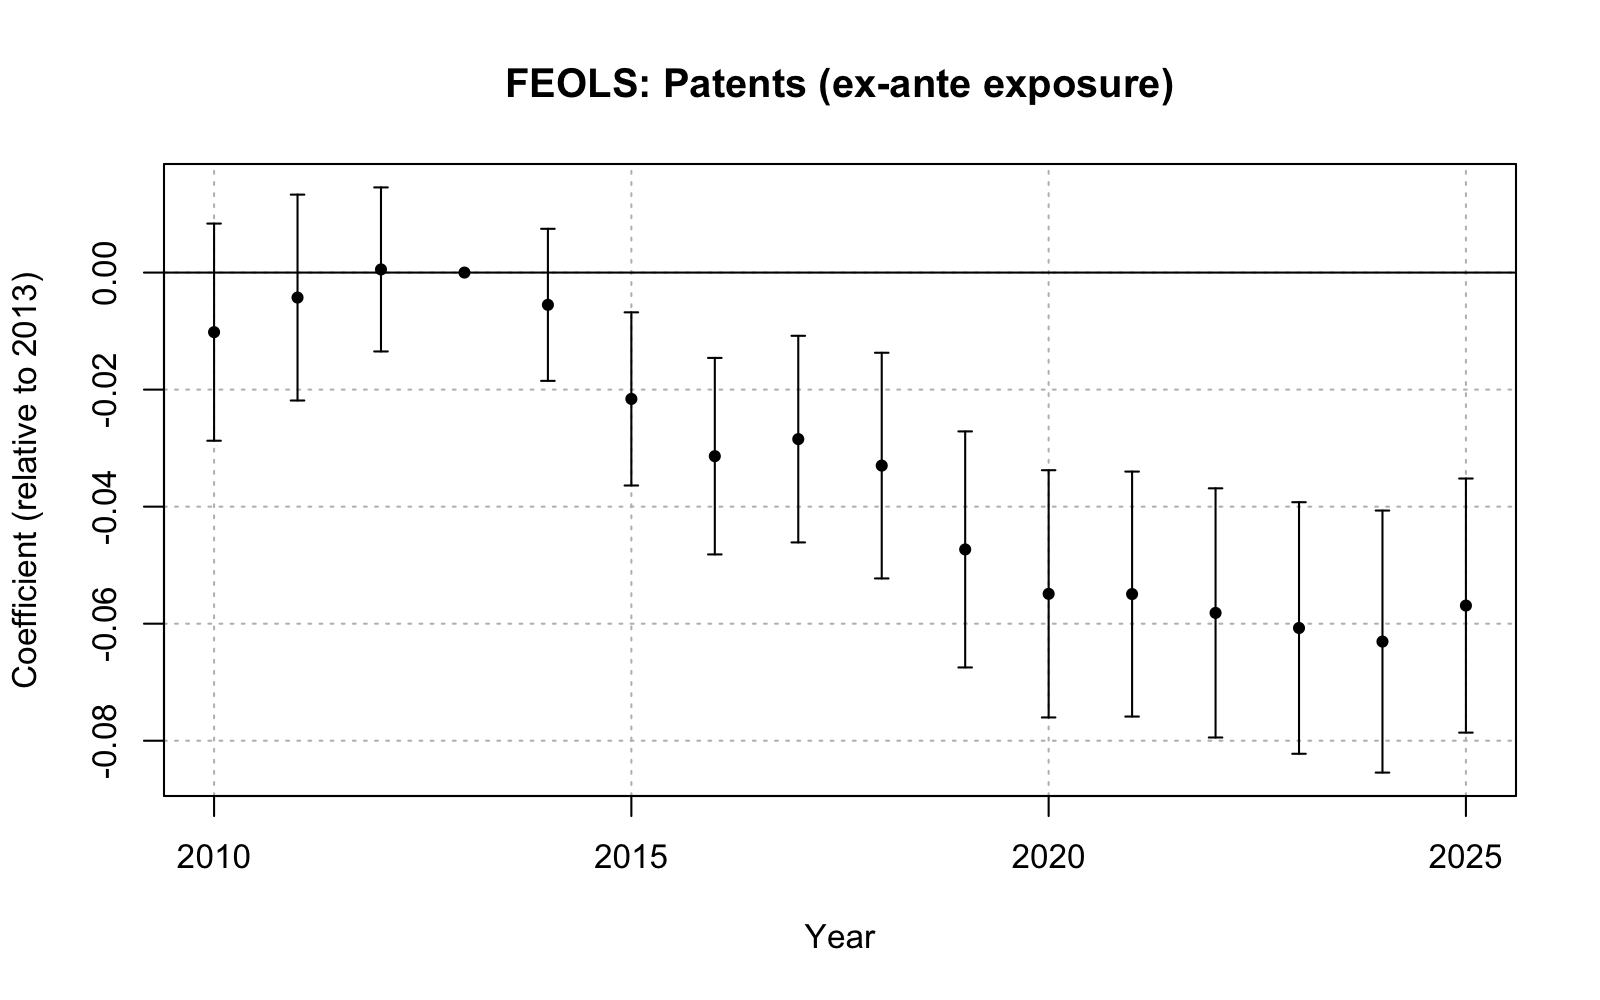
\includegraphics[width=\linewidth]{../output/RQ1/patent_feols_exante.png}
  \caption{FEOLS event study: patents, ex-ante Medicaid exposure}
  \label{fig:rq1_patent_feols_exante}
\end{figure}

\begin{figure}[!h]
  \centering
  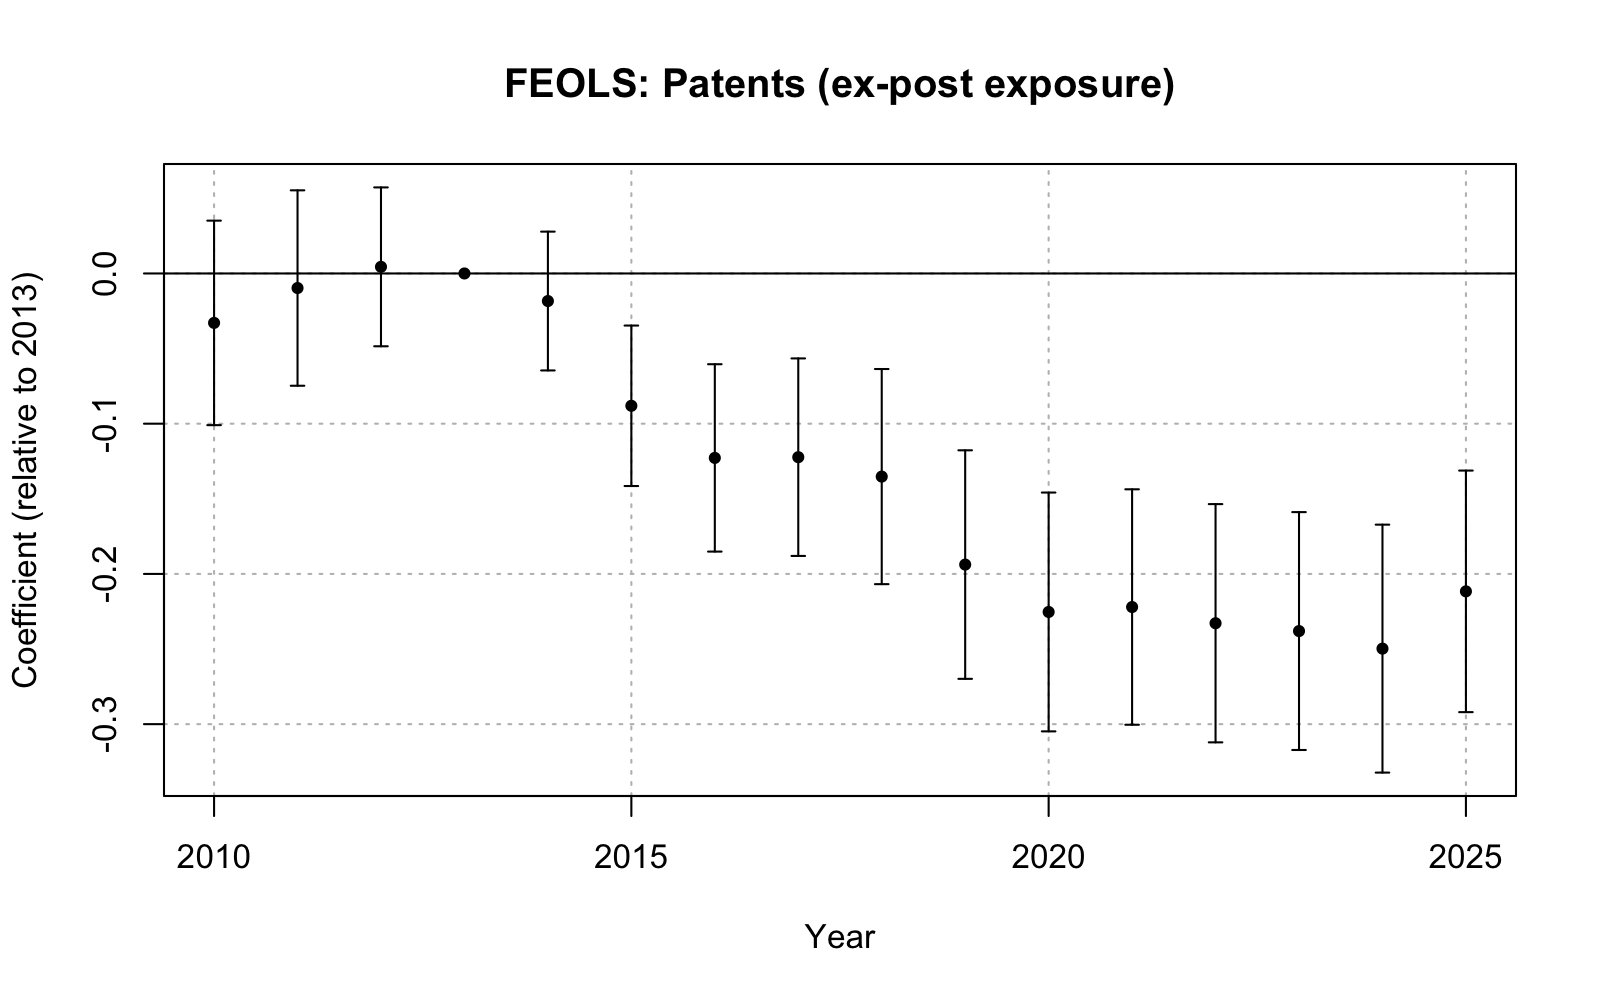
\includegraphics[width=\linewidth]{../output/RQ1/patent_feols_expost.png}
  \caption{FEOLS event study: patents, ex-post Medicaid exposure}
  \label{fig:rq1_patent_feols_expost}
\end{figure}

\begin{figure}[!h]
  \centering
  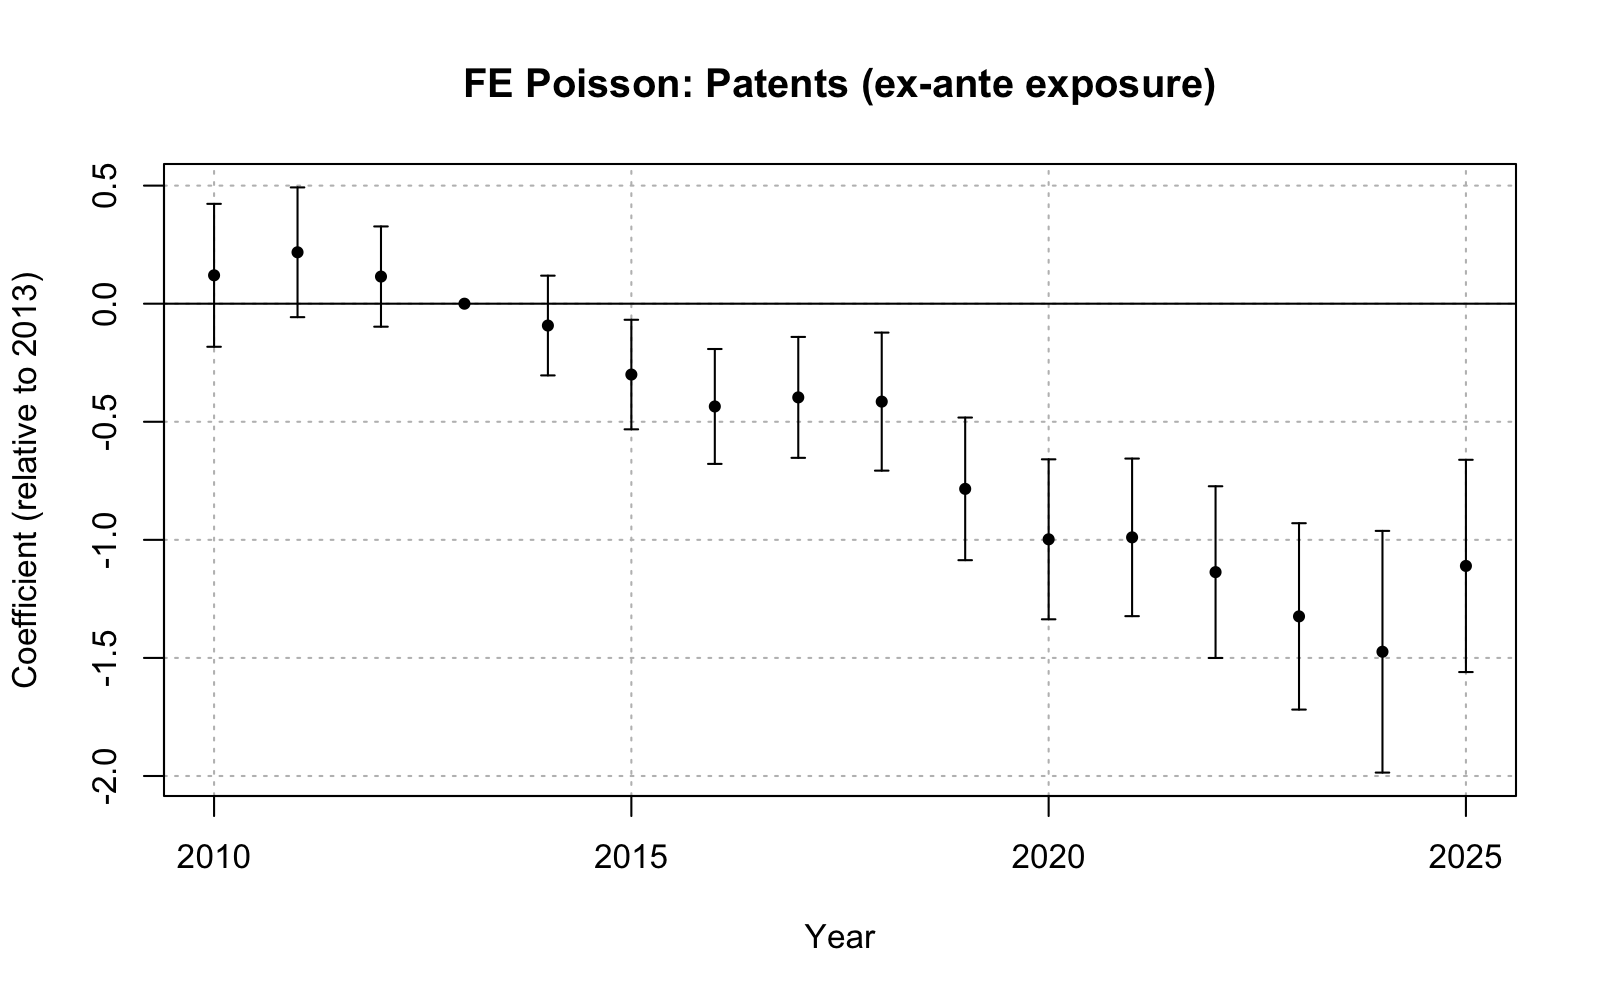
\includegraphics[width=\linewidth]{../output/RQ1/patent_poi_exante.png}
  \caption{FE Poisson event study: patents, ex-ante Medicaid exposure}
  \label{fig:rq1_patent_poi_exante}
\end{figure}

\begin{figure}[!h]
  \centering
  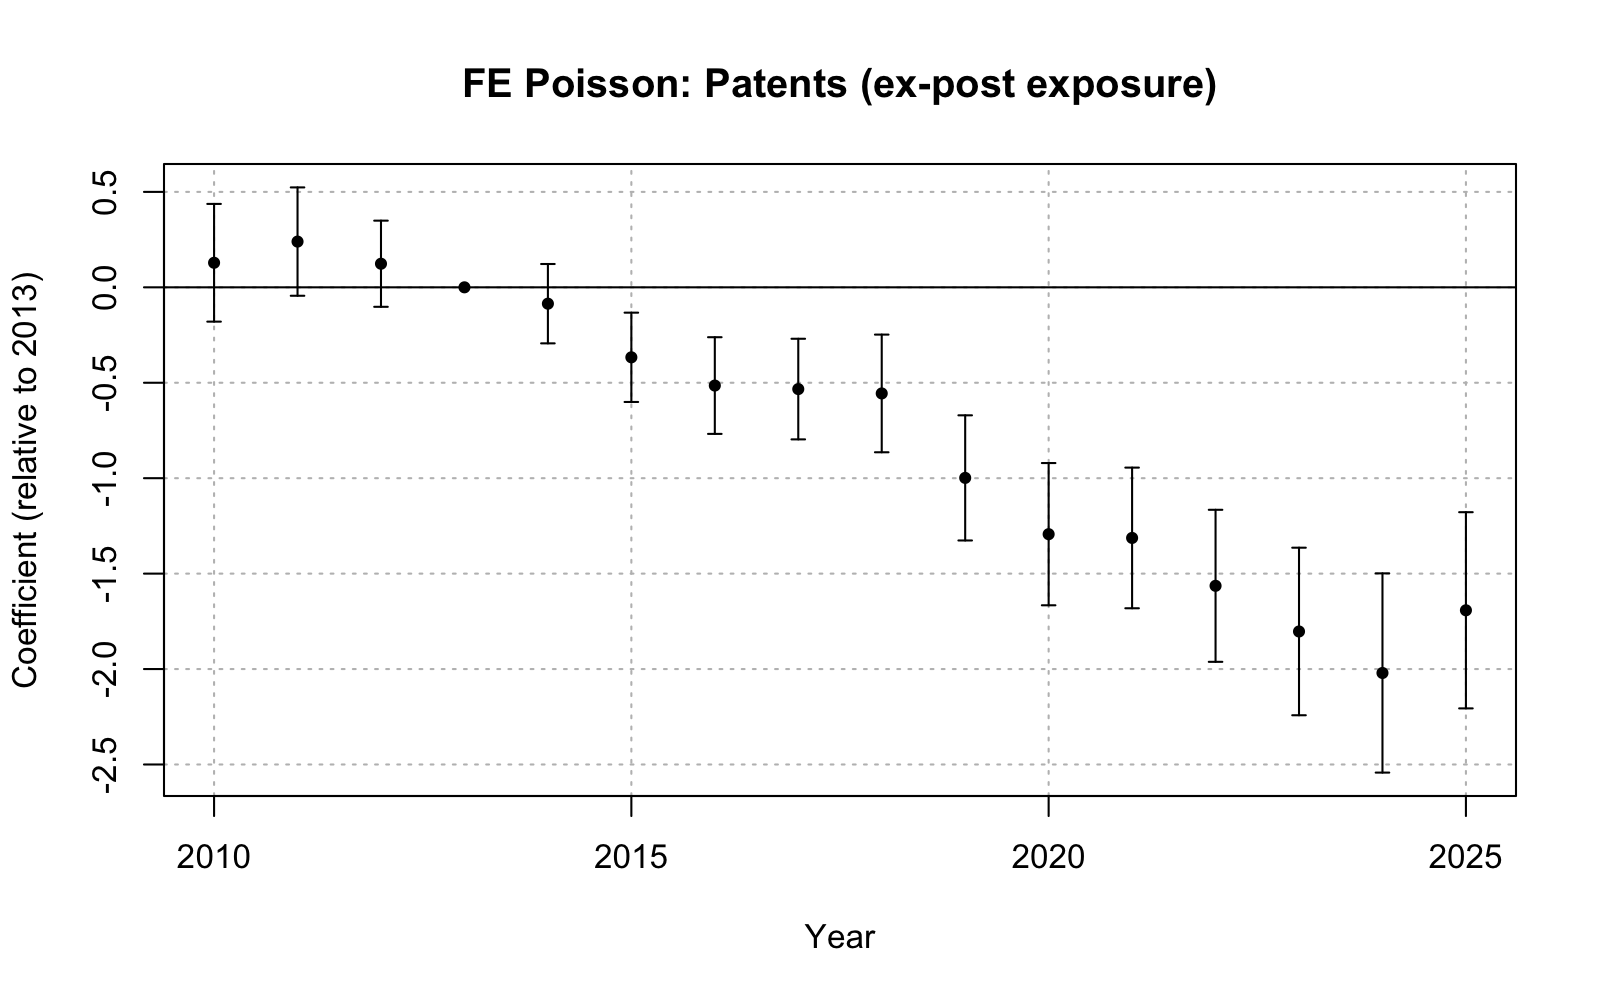
\includegraphics[width=\linewidth]{../output/RQ1/patent_poi_expost.png}
  \caption{FE Poisson event study: patents, ex-post Medicaid exposure}
  \label{fig:rq1_patent_poi_expost}
\end{figure}

\clearpage
\begingroup\footnotesize
\begin{table}
\centering
\begin{talltblr}[         %% tabularray outer open
entry=none,label=none,
note{}={* p \num{< 0.05}, ** p \num{< 0.01}, *** p \num{< 0.001}},
]                     %% tabularray outer close
{                     %% tabularray inner open
colspec={Q[]Q[]Q[]Q[]Q[]},
column{2,3,4,5}={}{halign=c,},
column{1}={}{halign=l,},
hline{32}={1,2,3,4,5}{solid, black, 0.05em},
}                     %% tabularray inner close
\toprule
& FEOLS: Ex Ante & FEOLS: Ex Post & FEPOIS: Ex Ante & FEPOIS: Ex Post \\ \midrule %% TinyTableHeader
2010 × medicaid\_market\_share & \num{-0.010}    & \num{-0.008}    & \num{0.120}     & \num{0.129}     \\
                                              & (\num{0.009})   & (\num{0.009})   & (\num{0.154})   & (\num{0.157})   \\
2011 × medicaid\_market\_share & \num{-0.004}    & \num{-0.002}    & \num{0.218}     & \num{0.240}     \\
                                              & (\num{0.009})   & (\num{0.008})   & (\num{0.140})   & (\num{0.145})   \\
2012 × medicaid\_market\_share & \num{0.001}     & \num{0.001}     & \num{0.115}     & \num{0.124}     \\
                                              & (\num{0.007})   & (\num{0.007})   & (\num{0.108})   & (\num{0.115})   \\
2014 × medicaid\_market\_share & \num{-0.006}    & \num{-0.005}    & \num{-0.092}    & \num{-0.086}    \\
                                              & (\num{0.007})   & (\num{0.006})   & (\num{0.108})   & (\num{0.106})   \\
2015 × medicaid\_market\_share & \num{-0.022}**  & \num{-0.022}**  & \num{-0.300}*   & \num{-0.367}**  \\
                                              & (\num{0.008})   & (\num{0.007})   & (\num{0.118})   & (\num{0.119})   \\
2016 × medicaid\_market\_share & \num{-0.031}*** & \num{-0.031}*** & \num{-0.435}*** & \num{-0.515}*** \\
                                              & (\num{0.009})   & (\num{0.008})   & (\num{0.124})   & (\num{0.129})   \\
2017 × medicaid\_market\_share & \num{-0.028}**  & \num{-0.031}*** & \num{-0.397}**  & \num{-0.533}*** \\
                                              & (\num{0.009})   & (\num{0.008})   & (\num{0.131})   & (\num{0.134})   \\
2018 × medicaid\_market\_share & \num{-0.033}*** & \num{-0.034}*** & \num{-0.415}**  & \num{-0.556}*** \\
                                              & (\num{0.010})   & (\num{0.009})   & (\num{0.149})   & (\num{0.157})   \\
2019 × medicaid\_market\_share & \num{-0.047}*** & \num{-0.048}*** & \num{-0.784}*** & \num{-0.998}*** \\
                                              & (\num{0.010})   & (\num{0.010})   & (\num{0.154})   & (\num{0.167})   \\
2020 × medicaid\_market\_share & \num{-0.055}*** & \num{-0.056}*** & \num{-0.998}*** & \num{-1.293}*** \\
                                              & (\num{0.011})   & (\num{0.010})   & (\num{0.173})   & (\num{0.190})   \\
2021 × medicaid\_market\_share & \num{-0.055}*** & \num{-0.056}*** & \num{-0.989}*** & \num{-1.313}*** \\
                                              & (\num{0.011})   & (\num{0.010})   & (\num{0.170})   & (\num{0.188})   \\
2022 × medicaid\_market\_share & \num{-0.058}*** & \num{-0.058}*** & \num{-1.137}*** & \num{-1.564}*** \\
                                              & (\num{0.011})   & (\num{0.010})   & (\num{0.186})   & (\num{0.203})   \\
2023 × medicaid\_market\_share & \num{-0.061}*** & \num{-0.060}*** & \num{-1.324}*** & \num{-1.803}*** \\
                                              & (\num{0.011})   & (\num{0.010})   & (\num{0.201})   & (\num{0.224})   \\
2024 × medicaid\_market\_share & \num{-0.063}*** & \num{-0.062}*** & \num{-1.474}*** & \num{-2.021}*** \\
                                              & (\num{0.011})   & (\num{0.011})   & (\num{0.261})   & (\num{0.266})   \\
2025 × medicaid\_market\_share & \num{-0.057}*** & \num{-0.053}*** & \num{-1.110}*** & \num{-1.692}*** \\
                                              & (\num{0.011})   & (\num{0.010})   & (\num{0.229})   & (\num{0.262})   \\
Num. obs.                                     & \num{21126784}  & \num{21126784}  & \num{5203776}   & \num{5203776}   \\
R2                                            & \num{0.392}     & \num{0.392}     &                 &                 \\
\bottomrule
\end{talltblr}
\end{table}

\endgroup

\clearpage

\subsection{FDA Approvals}

\begin{figure}[!h]
  \centering
  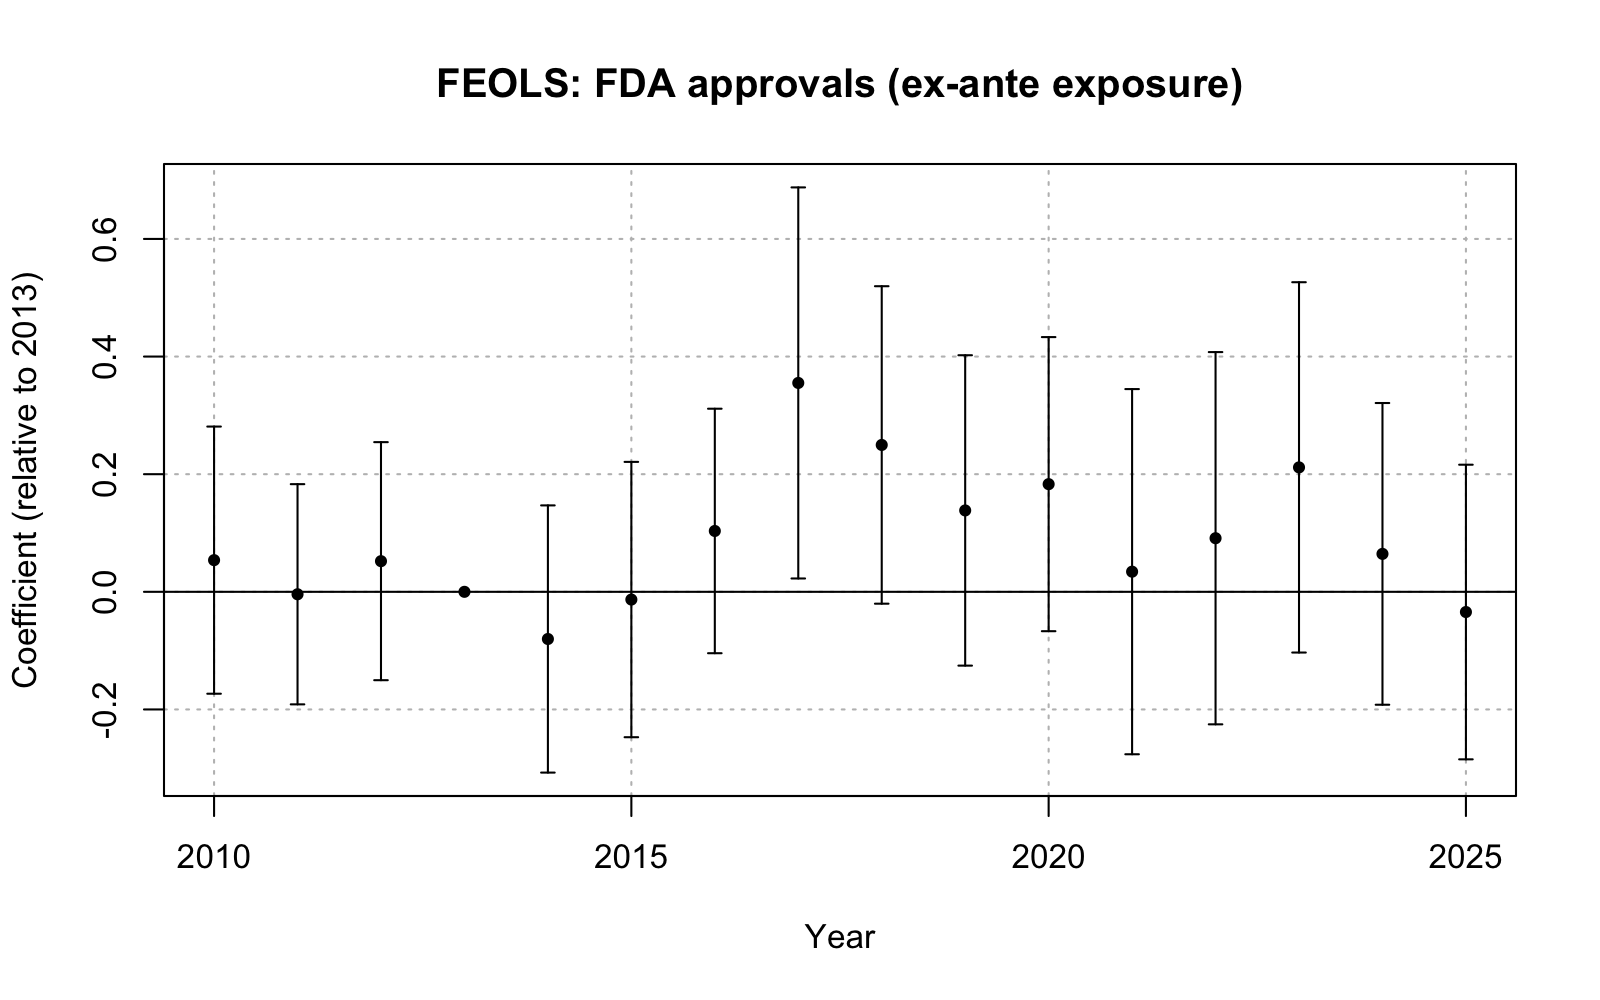
\includegraphics[width=\linewidth]{../output/RQ1/fda_feols_exante.png}
  \caption{FEOLS event study: FDA approvals, ex-ante Medicaid exposure}
  \label{fig:rq1_fda_feols_exante}
\end{figure}

\begin{figure}[!h]
  \centering
  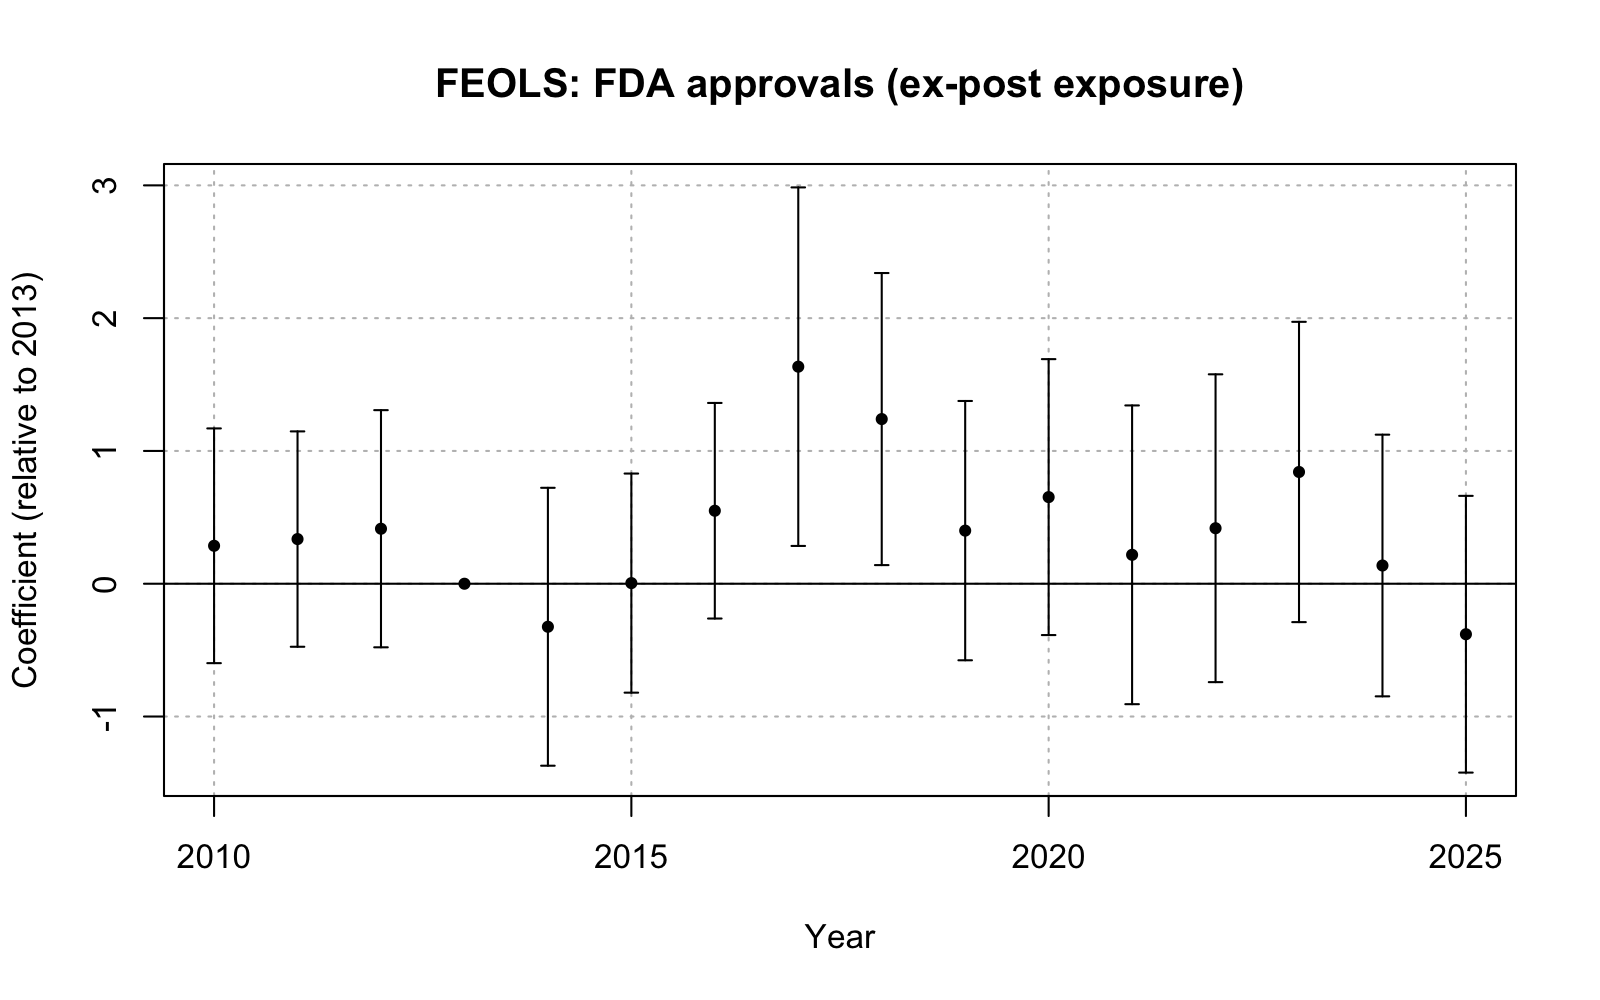
\includegraphics[width=\linewidth]{../output/RQ1/fda_feols_expost.png}
  \caption{FEOLS event study: FDA approvals, ex-post Medicaid exposure}
  \label{fig:rq1_fda_feols_expost}
\end{figure}

\begin{figure}[!h]
  \centering
  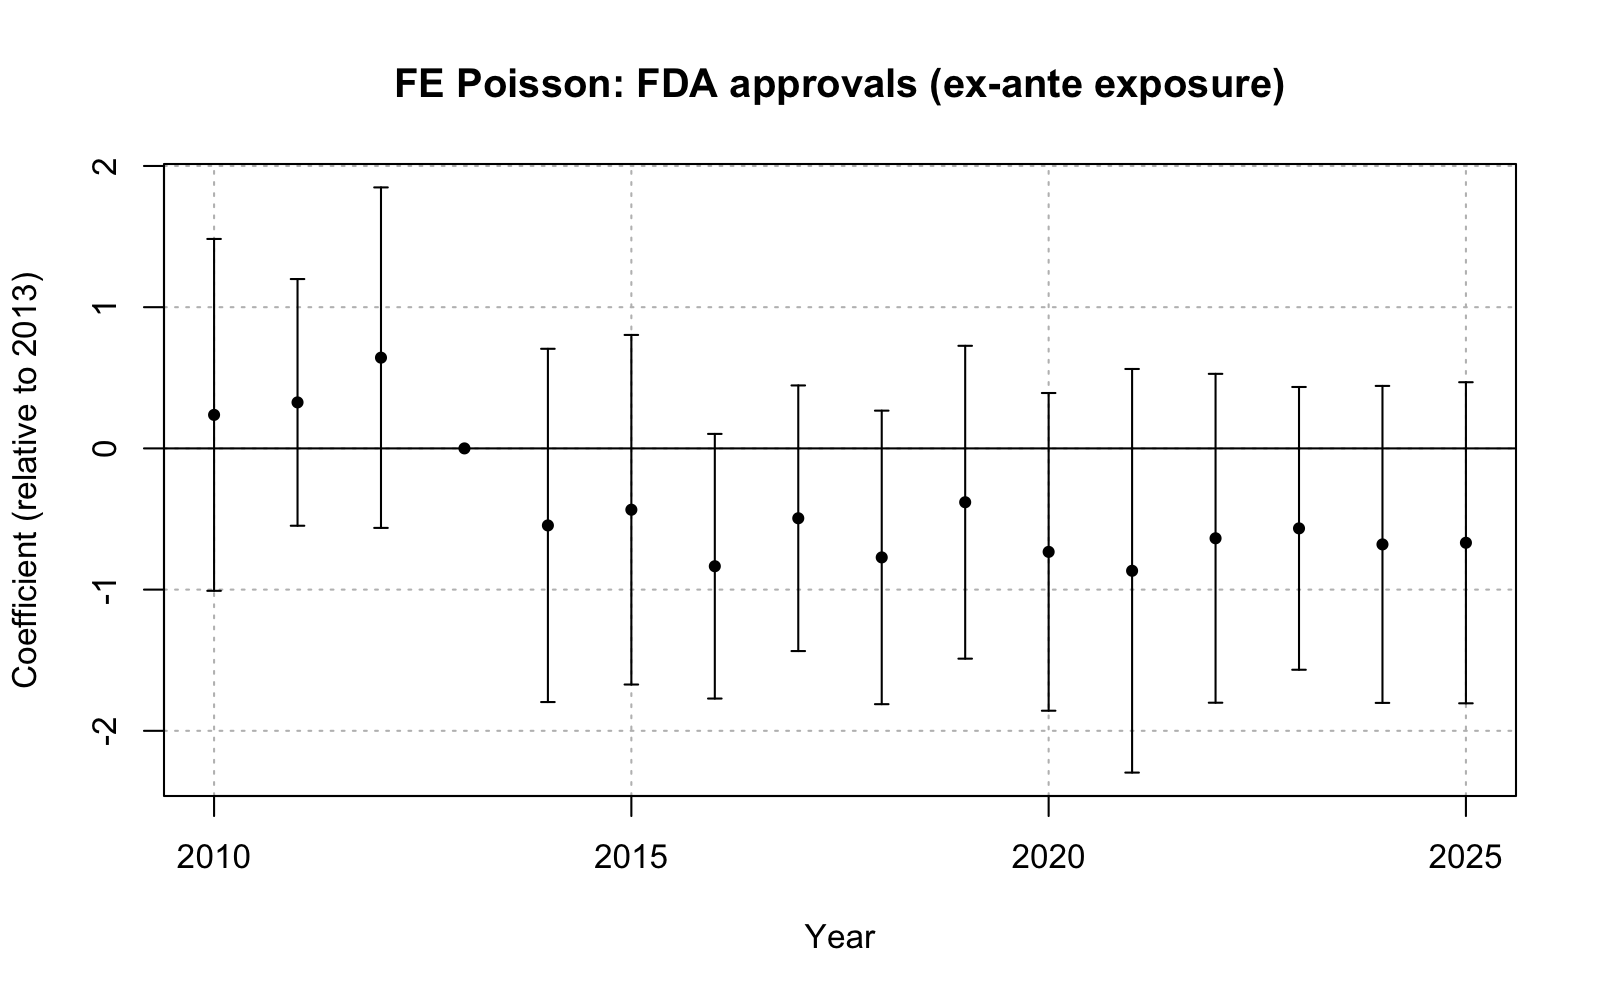
\includegraphics[width=\linewidth]{../output/RQ1/fda_poi_exante.png}
  \caption{FE Poisson event study: FDA approvals, ex-ante Medicaid exposure}
  \label{fig:rq1_fda_poi_exante}
\end{figure}

\begin{figure}[!h]
  \centering
  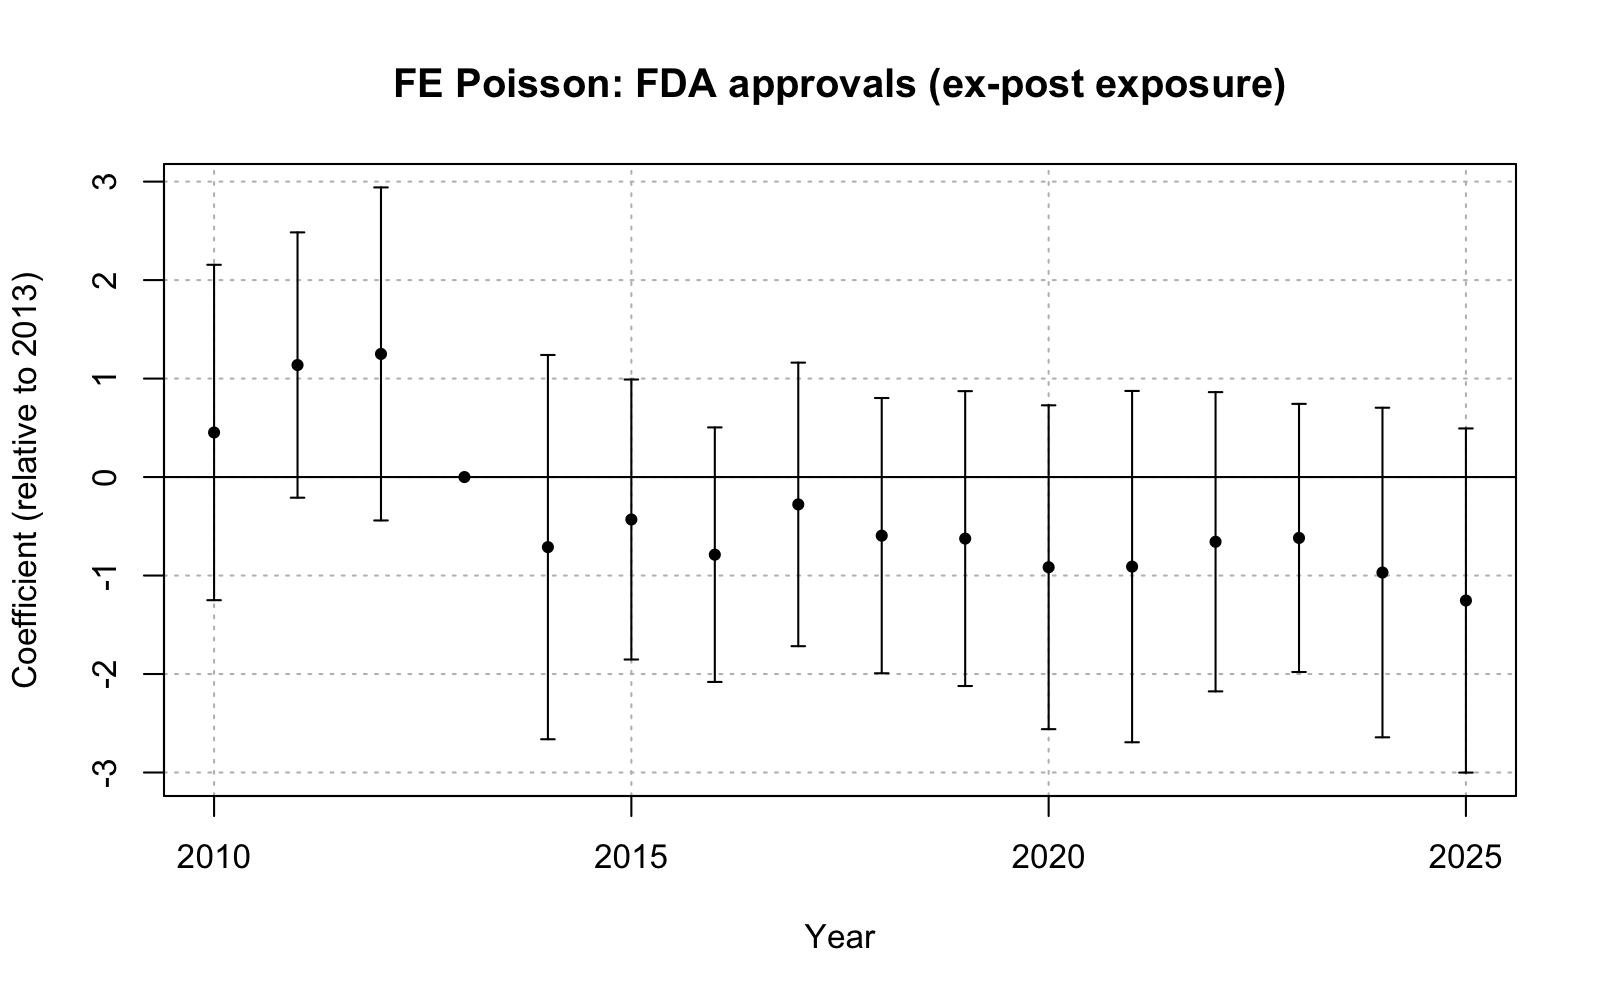
\includegraphics[width=\linewidth]{../output/RQ1/fda_poi_expost.png}
  \caption{FE Poisson event study: FDA approvals, ex-post Medicaid exposure}
  \label{fig:rq1_fda_poi_expost}
\end{figure}

\clearpage
\begingroup\footnotesize
\begin{table}
\centering
\begin{talltblr}[         %% tabularray outer open
entry=none,label=none,
note{}={* p \num{< 0.05}, ** p \num{< 0.01}, *** p \num{< 0.001}},
]                     %% tabularray outer close
{                     %% tabularray inner open
colspec={Q[]Q[]Q[]Q[]Q[]},
column{2,3,4,5}={}{halign=c,},
column{1}={}{halign=l,},
hline{32}={1,2,3,4,5}{solid, black, 0.05em},
}                     %% tabularray inner close
\toprule
& FEOLS: Ex Ante & FEOLS: Ex Post & FEPOIS: Ex Ante & FEPOIS: Ex Post \\ \midrule %% TinyTableHeader
2010 × medicaid\_market\_share & \num{0.054}   & \num{0.071}   & \num{0.237}   & \num{0.453}   \\
& (\num{0.116}) & (\num{0.113}) & (\num{0.636}) & (\num{0.869}) \\
2011 × medicaid\_market\_share & \num{-0.004}  & \num{0.084}   & \num{0.326}   & \num{1.138}   \\
& (\num{0.095}) & (\num{0.103}) & (\num{0.446}) & (\num{0.687}) \\
2012 × medicaid\_market\_share & \num{0.052}   & \num{0.104}   & \num{0.643}   & \num{1.250}   \\
& (\num{0.103}) & (\num{0.114}) & (\num{0.615}) & (\num{0.863}) \\
2014 × medicaid\_market\_share & \num{-0.080}  & \num{-0.081}  & \num{-0.545}  & \num{-0.711}  \\
& (\num{0.116}) & (\num{0.133}) & (\num{0.638}) & (\num{0.995}) \\
2015 × medicaid\_market\_share & \num{-0.013}  & \num{0.001}   & \num{-0.434}  & \num{-0.431}  \\
& (\num{0.119}) & (\num{0.105}) & (\num{0.631}) & (\num{0.725}) \\
2016 × medicaid\_market\_share & \num{0.103}   & \num{0.137}   & \num{-0.834}  & \num{-0.788}  \\
& (\num{0.106}) & (\num{0.103}) & (\num{0.478}) & (\num{0.659}) \\
2017 × medicaid\_market\_share & \num{0.355}*  & \num{0.409}*  & \num{-0.495}  & \num{-0.278}  \\
& (\num{0.169}) & (\num{0.172}) & (\num{0.480}) & (\num{0.735}) \\
2018 × medicaid\_market\_share & \num{0.250}   & \num{0.310}*  & \num{-0.772}  & \num{-0.595}  \\
& (\num{0.137}) & (\num{0.140}) & (\num{0.530}) & (\num{0.713}) \\
2019 × medicaid\_market\_share & \num{0.138}   & \num{0.100}   & \num{-0.381}  & \num{-0.625}  \\
& (\num{0.134}) & (\num{0.124}) & (\num{0.565}) & (\num{0.764}) \\
2020 × medicaid\_market\_share & \num{0.183}   & \num{0.163}   & \num{-0.733}  & \num{-0.916}  \\
& (\num{0.127}) & (\num{0.132}) & (\num{0.574}) & (\num{0.839}) \\
2021 × medicaid\_market\_share & \num{0.034}   & \num{0.054}   & \num{-0.867}  & \num{-0.909}  \\
& (\num{0.158}) & (\num{0.143}) & (\num{0.729}) & (\num{0.910}) \\
2022 × medicaid\_market\_share & \num{0.091}   & \num{0.104}   & \num{-0.637}  & \num{-0.657}  \\
& (\num{0.161}) & (\num{0.148}) & (\num{0.594}) & (\num{0.775}) \\
2023 × medicaid\_market\_share & \num{0.212}   & \num{0.210}   & \num{-0.566}  & \num{-0.618}  \\
& (\num{0.160}) & (\num{0.144}) & (\num{0.511}) & (\num{0.695}) \\
2024 × medicaid\_market\_share & \num{0.065}   & \num{0.034}   & \num{-0.680}  & \num{-0.969}  \\
& (\num{0.131}) & (\num{0.125}) & (\num{0.573}) & (\num{0.854}) \\
2025 × medicaid\_market\_share & \num{-0.034}  & \num{-0.095}  & \num{-0.668}  & \num{-1.254}  \\
& (\num{0.128}) & (\num{0.133}) & (\num{0.580}) & (\num{0.892}) \\
Num. obs.                                          & \num{604800}  & \num{604800}  & \num{168704}  & \num{168704}  \\
R2                                                 & \num{0.314}   & \num{0.314}   &                &                \\
\bottomrule
\end{talltblr}
\end{table}

\endgroup

\clearpage

% -----------------------------------------------------------------------
\section{RQ2: Medicaid Demand and PDL Exposure}
% -----------------------------------------------------------------------

\subsection{Patents}

\begin{figure}[!h]
  \centering
  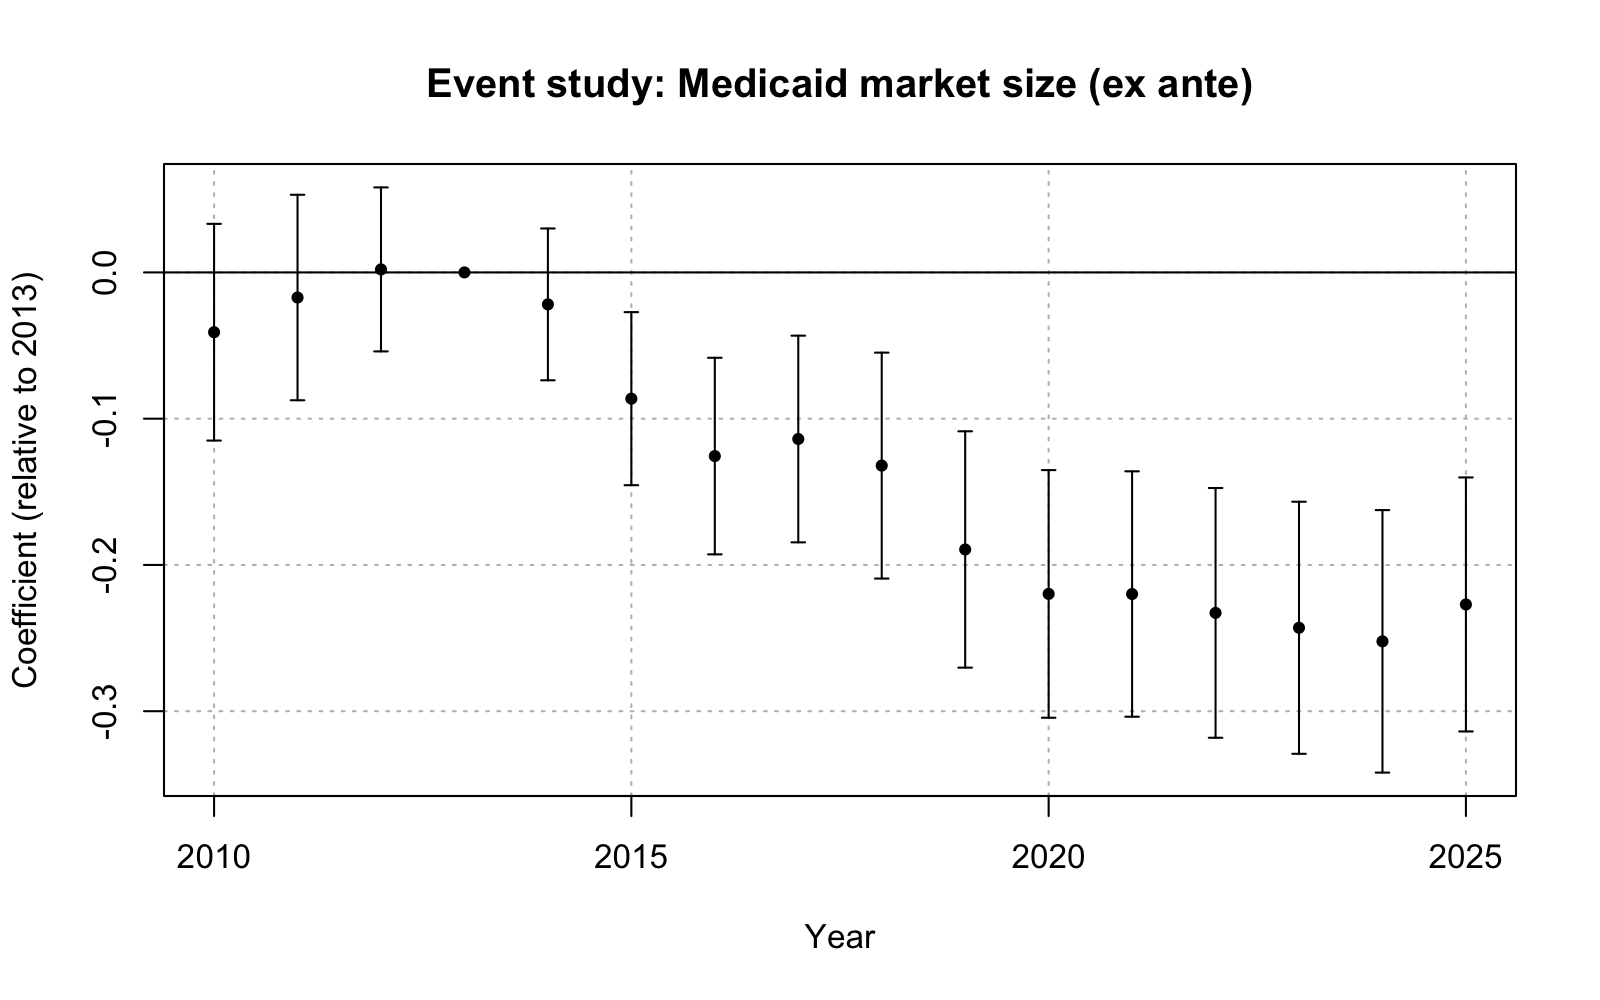
\includegraphics[width=\linewidth]{../output/RQ2/patent_feols_exante_medicaid.png}
  \caption{FEOLS event study: patents, Medicaid exposure (ex-ante)}
  \label{fig:rq2_patent_feols_exante_medicaid}
\end{figure}

\begin{figure}[!h]
  \centering
  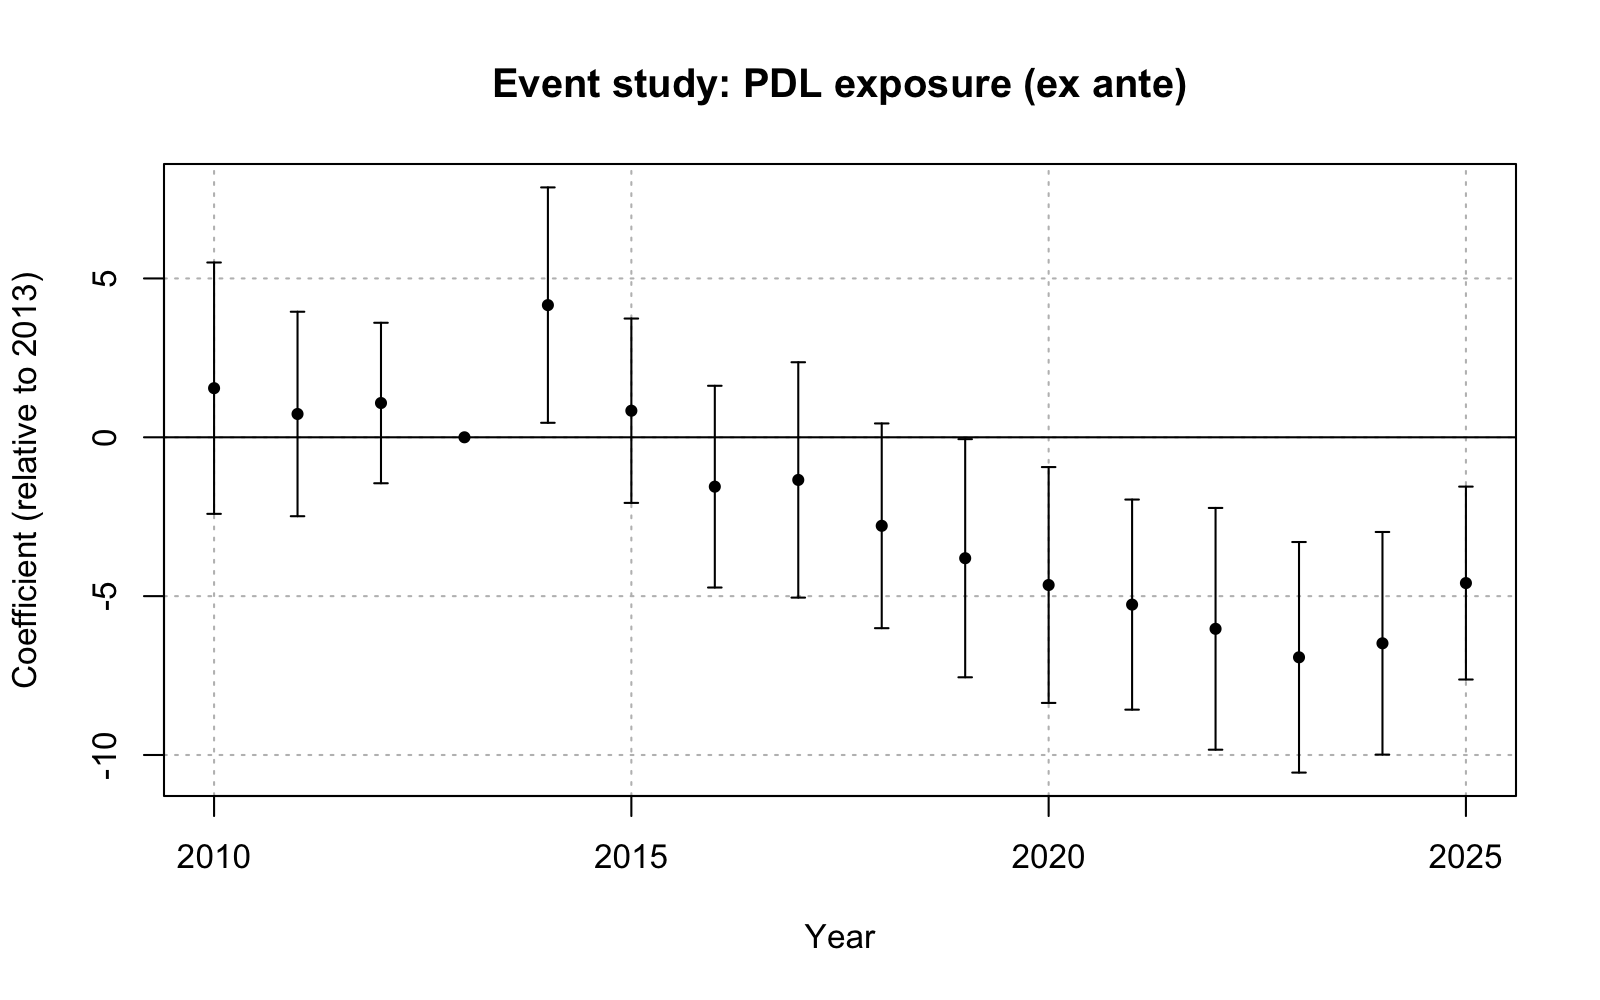
\includegraphics[width=\linewidth]{../output/RQ2/patent_feols_exante_pdl.png}
  \caption{FEOLS event study: patents, PDL exposure (ex-ante)}
  \label{fig:rq2_patent_feols_exante_pdl}
\end{figure}

\begin{figure}[!h]
  \centering
  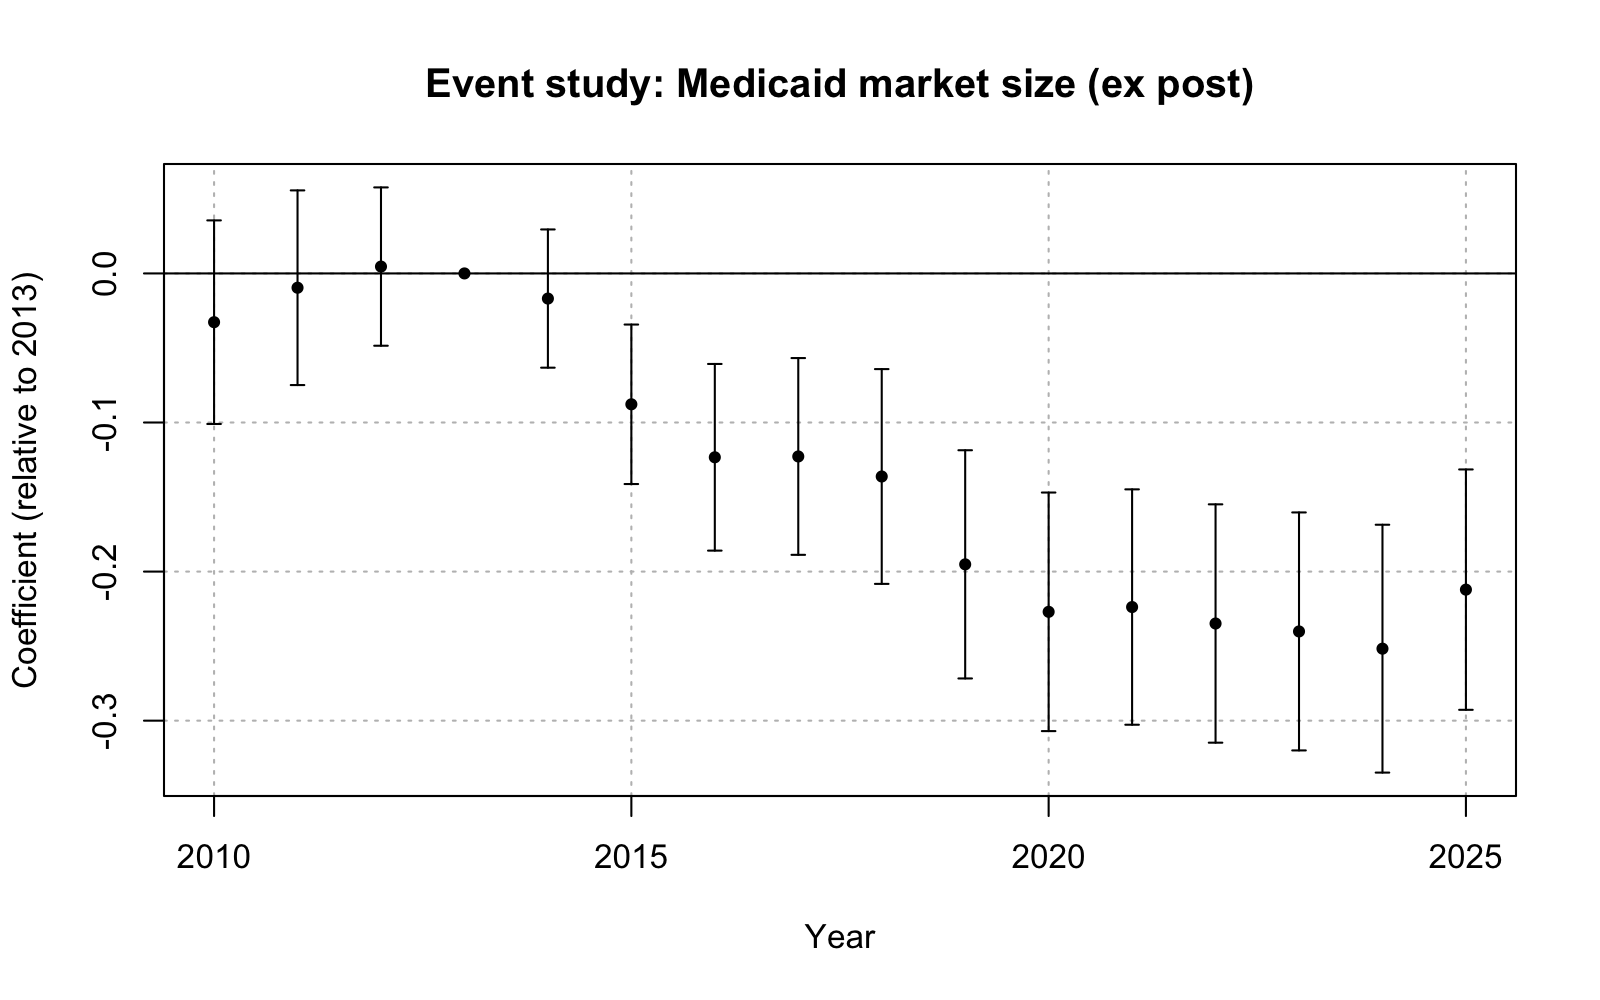
\includegraphics[width=\linewidth]{../output/RQ2/patent_feols_expost_medicaid.png}
  \caption{FEOLS event study: patents, Medicaid exposure (ex-post)}
  \label{fig:rq2_patent_feols_expost_medicaid}
\end{figure}

\begin{figure}[!h]
  \centering
  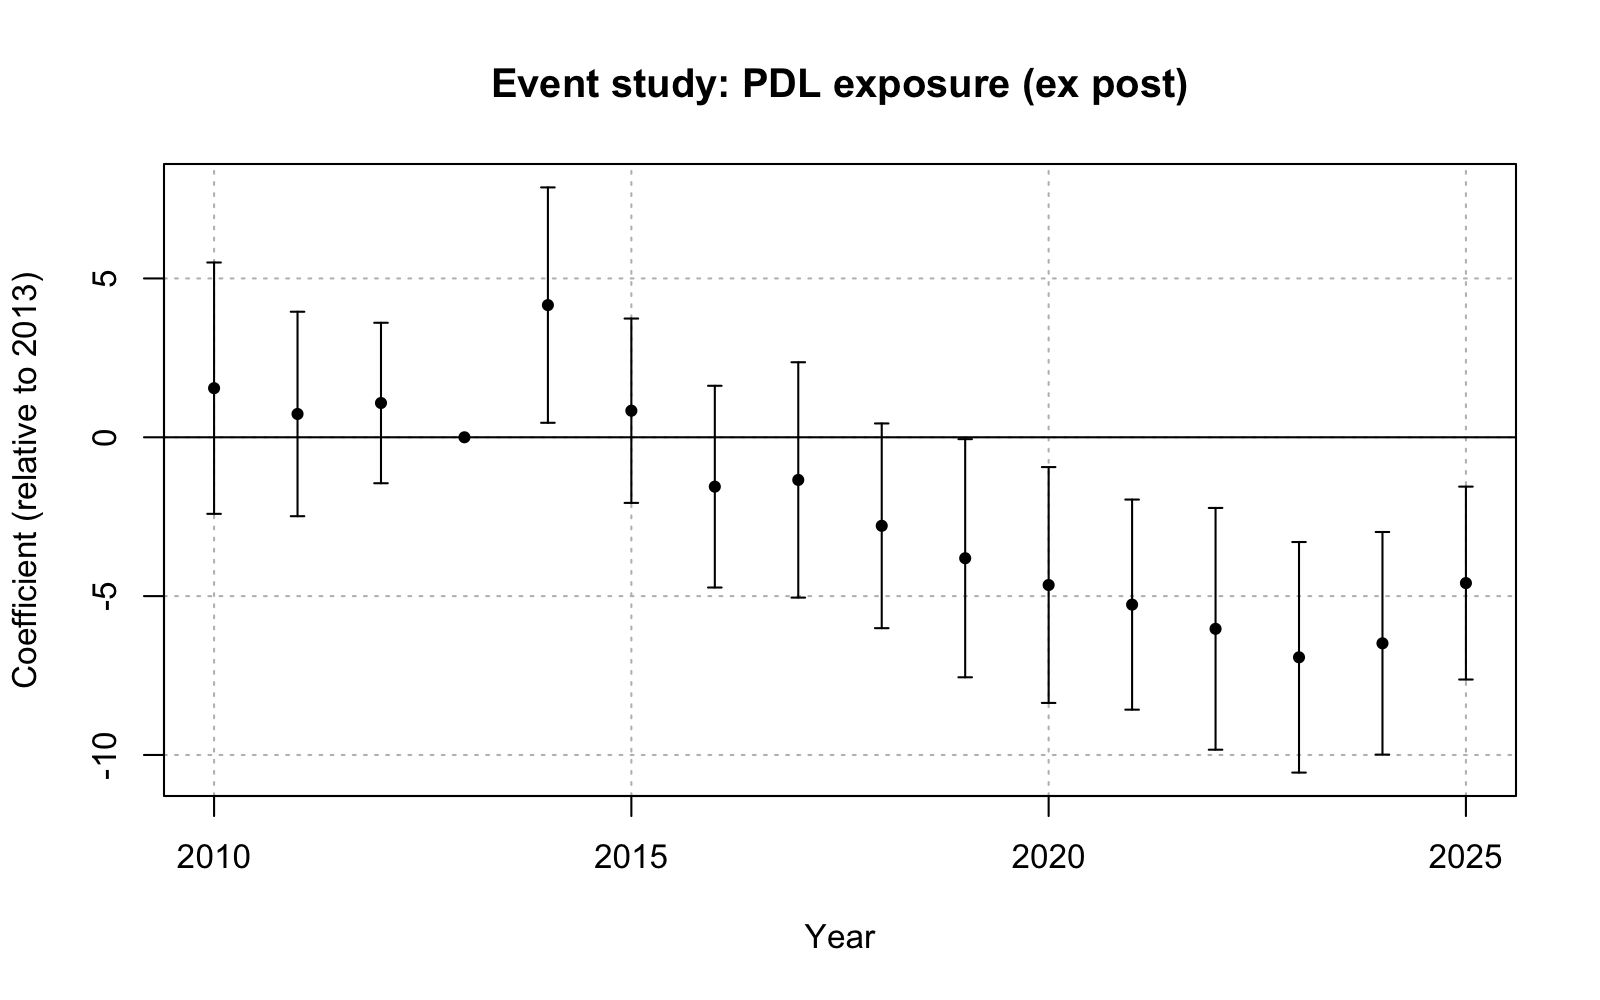
\includegraphics[width=\linewidth]{../output/RQ2/patent_feols_expost_pdl.png}
  \caption{FEOLS event study: patents, PDL exposure (ex-post)}
  \label{fig:rq2_patent_feols_expost_pdl}
\end{figure}

\clearpage
\begingroup\footnotesize
\begin{table}
\centering
\begin{talltblr}[         %% tabularray outer open
entry=none,label=none,
note{}={* p \num{< 0.05}, ** p \num{< 0.01}, *** p \num{< 0.001}},
]                     %% tabularray outer close
{                     %% tabularray inner open
colspec={Q[]Q[]Q[]},
column{2,3}={}{halign=c,},
column{1}={}{halign=l,},
hline{62}={1,2,3}{solid, black, 0.05em},
}                     %% tabularray inner close
\toprule
& FEOLS: Ex Ante & FEOLS: Ex Post \\ \midrule %% TinyTableHeader
2010 × medicaid\_market\_share & \num{-0.041}    & \num{-0.033}    \\
& (\num{0.038})   & (\num{0.035})   \\
2011 × medicaid\_market\_share & \num{-0.017}    & \num{-0.010}    \\
& (\num{0.036})   & (\num{0.033})   \\
2012 × medicaid\_market\_share & \num{0.002}     & \num{0.005}     \\
& (\num{0.029})   & (\num{0.027})   \\
2014 × medicaid\_market\_share & \num{-0.022}    & \num{-0.017}    \\
& (\num{0.026})   & (\num{0.024})   \\
2015 × medicaid\_market\_share & \num{-0.086}**  & \num{-0.088}**  \\
& (\num{0.030})   & (\num{0.027})   \\
2016 × medicaid\_market\_share & \num{-0.126}*** & \num{-0.123}*** \\
& (\num{0.034})   & (\num{0.032})   \\
2017 × medicaid\_market\_share & \num{-0.114}**  & \num{-0.123}*** \\
& (\num{0.036})   & (\num{0.034})   \\
2018 × medicaid\_market\_share & \num{-0.132}*** & \num{-0.136}*** \\
& (\num{0.039})   & (\num{0.037})   \\
2019 × medicaid\_market\_share & \num{-0.189}*** & \num{-0.195}*** \\
& (\num{0.041})   & (\num{0.039})   \\
2020 × medicaid\_market\_share & \num{-0.220}*** & \num{-0.227}*** \\
& (\num{0.043})   & (\num{0.041})   \\
2021 × medicaid\_market\_share & \num{-0.220}*** & \num{-0.224}*** \\
& (\num{0.043})   & (\num{0.040})   \\
2022 × medicaid\_market\_share & \num{-0.233}*** & \num{-0.235}*** \\
& (\num{0.044})   & (\num{0.041})   \\
2023 × medicaid\_market\_share & \num{-0.243}*** & \num{-0.240}*** \\
& (\num{0.044})   & (\num{0.041})   \\
2024 × medicaid\_market\_share & \num{-0.252}*** & \num{-0.252}*** \\
& (\num{0.046})   & (\num{0.042})   \\
2025 × medicaid\_market\_share & \num{-0.227}*** & \num{-0.212}*** \\
& (\num{0.044})   & (\num{0.041})   \\
2010 × in\_pdl                  & \num{1.546}     & \num{1.546}     \\
& (\num{2.018})   & (\num{2.018})   \\
2011 × in\_pdl                  & \num{0.734}     & \num{0.734}     \\
& (\num{1.642})   & (\num{1.642})   \\
2012 × in\_pdl                  & \num{1.079}     & \num{1.079}     \\
& (\num{1.289})   & (\num{1.289})   \\
2014 × in\_pdl                  & \num{4.161}*    & \num{4.161}*    \\
& (\num{1.890})   & (\num{1.890})   \\
2015 × in\_pdl                  & \num{0.836}     & \num{0.836}     \\
& (\num{1.480})   & (\num{1.480})   \\
2016 × in\_pdl                  & \num{-1.554}    & \num{-1.554}    \\
& (\num{1.620})   & (\num{1.620})   \\
2017 × in\_pdl                  & \num{-1.342}    & \num{-1.342}    \\
& (\num{1.890})   & (\num{1.890})   \\
2018 × in\_pdl                  & \num{-2.786}    & \num{-2.787}    \\
& (\num{1.644})   & (\num{1.644})   \\
2019 × in\_pdl                  & \num{-3.806}*   & \num{-3.807}*   \\
& (\num{1.912})   & (\num{1.912})   \\
2020 × in\_pdl                  & \num{-4.649}*   & \num{-4.650}*   \\
& (\num{1.894})   & (\num{1.894})   \\
2021 × in\_pdl                  & \num{-5.266}**  & \num{-5.267}**  \\
& (\num{1.687})   & (\num{1.687})   \\
2022 × in\_pdl                  & \num{-6.029}**  & \num{-6.029}**  \\
& (\num{1.941})   & (\num{1.941})   \\
2023 × in\_pdl                  & \num{-6.925}*** & \num{-6.926}*** \\
& (\num{1.851})   & (\num{1.851})   \\
2024 × in\_pdl                  & \num{-6.484}*** & \num{-6.485}*** \\
& (\num{1.788})   & (\num{1.788})   \\
2025 × in\_pdl                  & \num{-4.588}**  & \num{-4.589}**  \\
& (\num{1.549})   & (\num{1.549})   \\
Num. obs.                                        & \num{5281696}   & \num{5281696}   \\
R2                                               & \num{0.535}     & \num{0.535}     \\
\bottomrule
\end{talltblr}
\end{table}

\endgroup

\clearpage

\subsection{FDA Approvals}

\begin{figure}[!h]
  \centering
  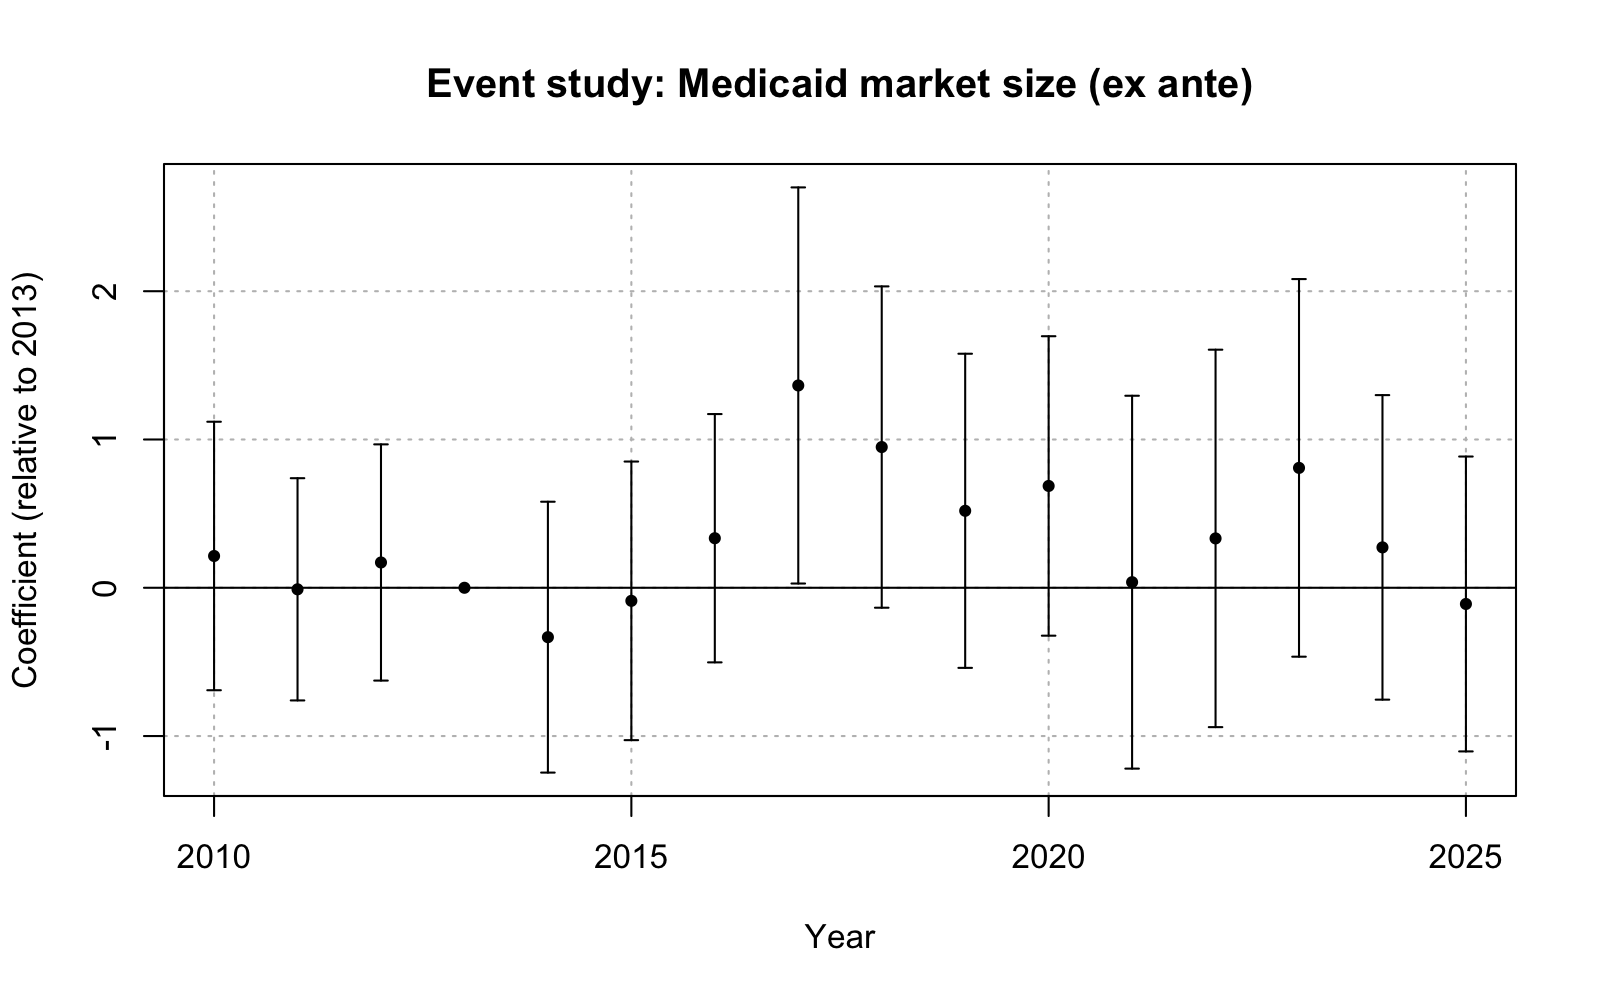
\includegraphics[width=\linewidth]{../output/RQ2/fda_feols_exante_medicaid.png}
  \caption{FEOLS event study: FDA approvals, Medicaid exposure (ex-ante)}
  \label{fig:rq2_fda_feols_exante_medicaid}
\end{figure}

\begin{figure}[!h]
  \centering
  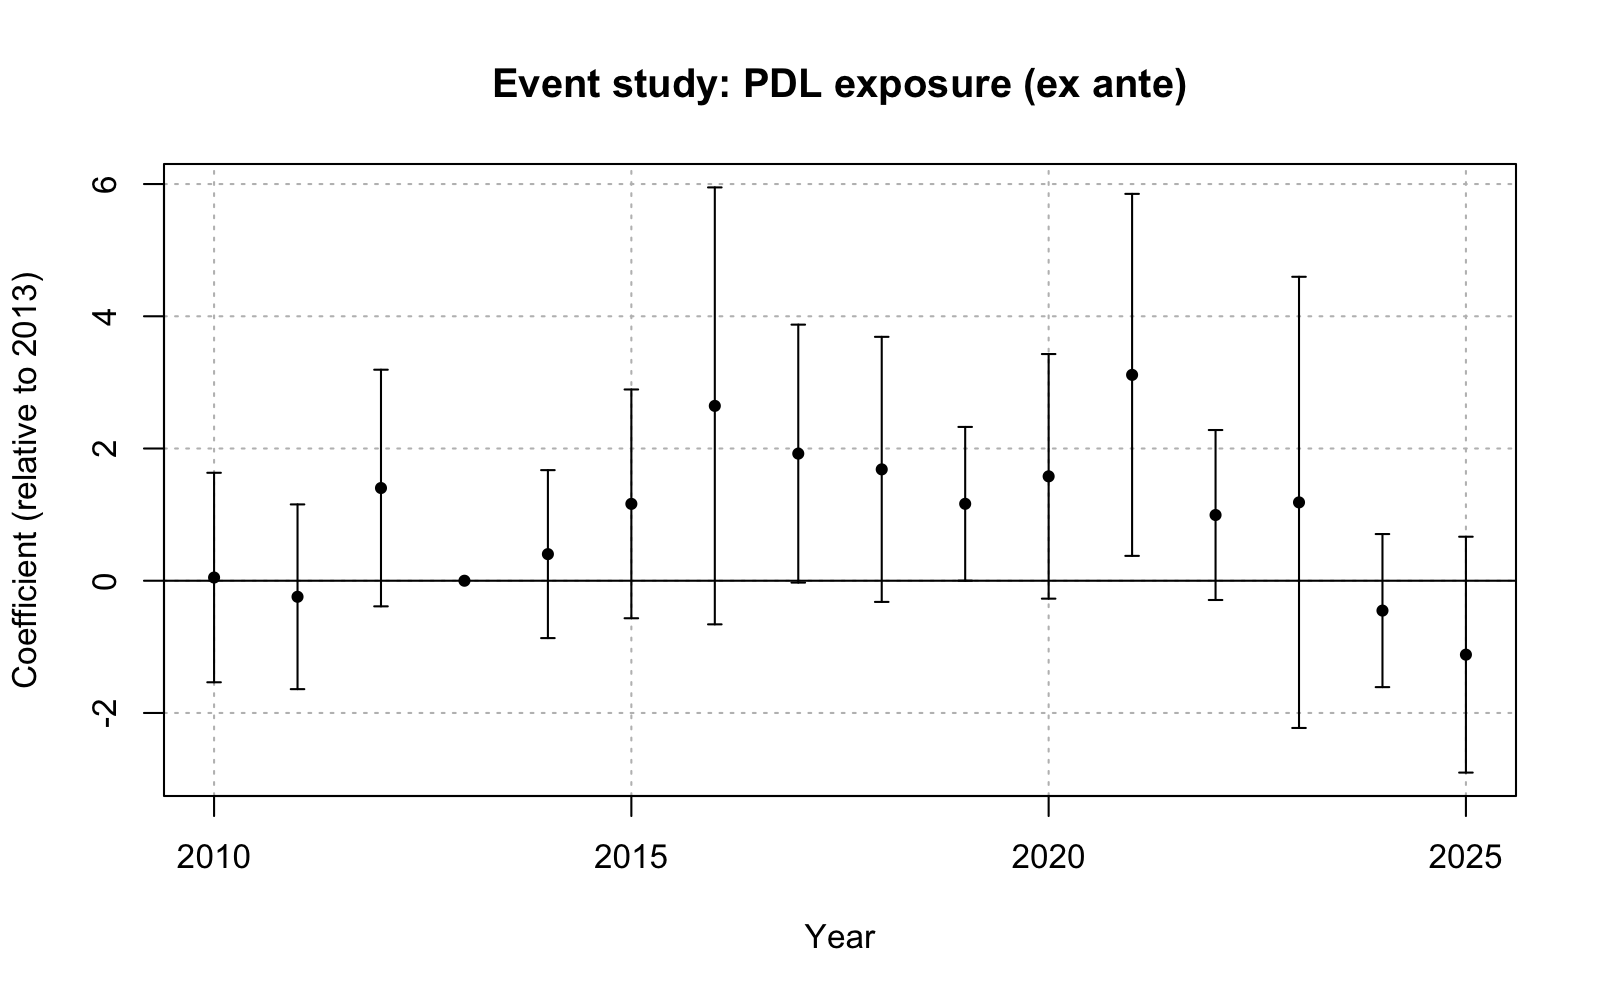
\includegraphics[width=\linewidth]{../output/RQ2/fda_feols_exante_pdl.png}
  \caption{FEOLS event study: FDA approvals, PDL exposure (ex-ante)}
  \label{fig:rq2_fda_feols_exante_pdl}
\end{figure}

\begin{figure}[!h]
  \centering
  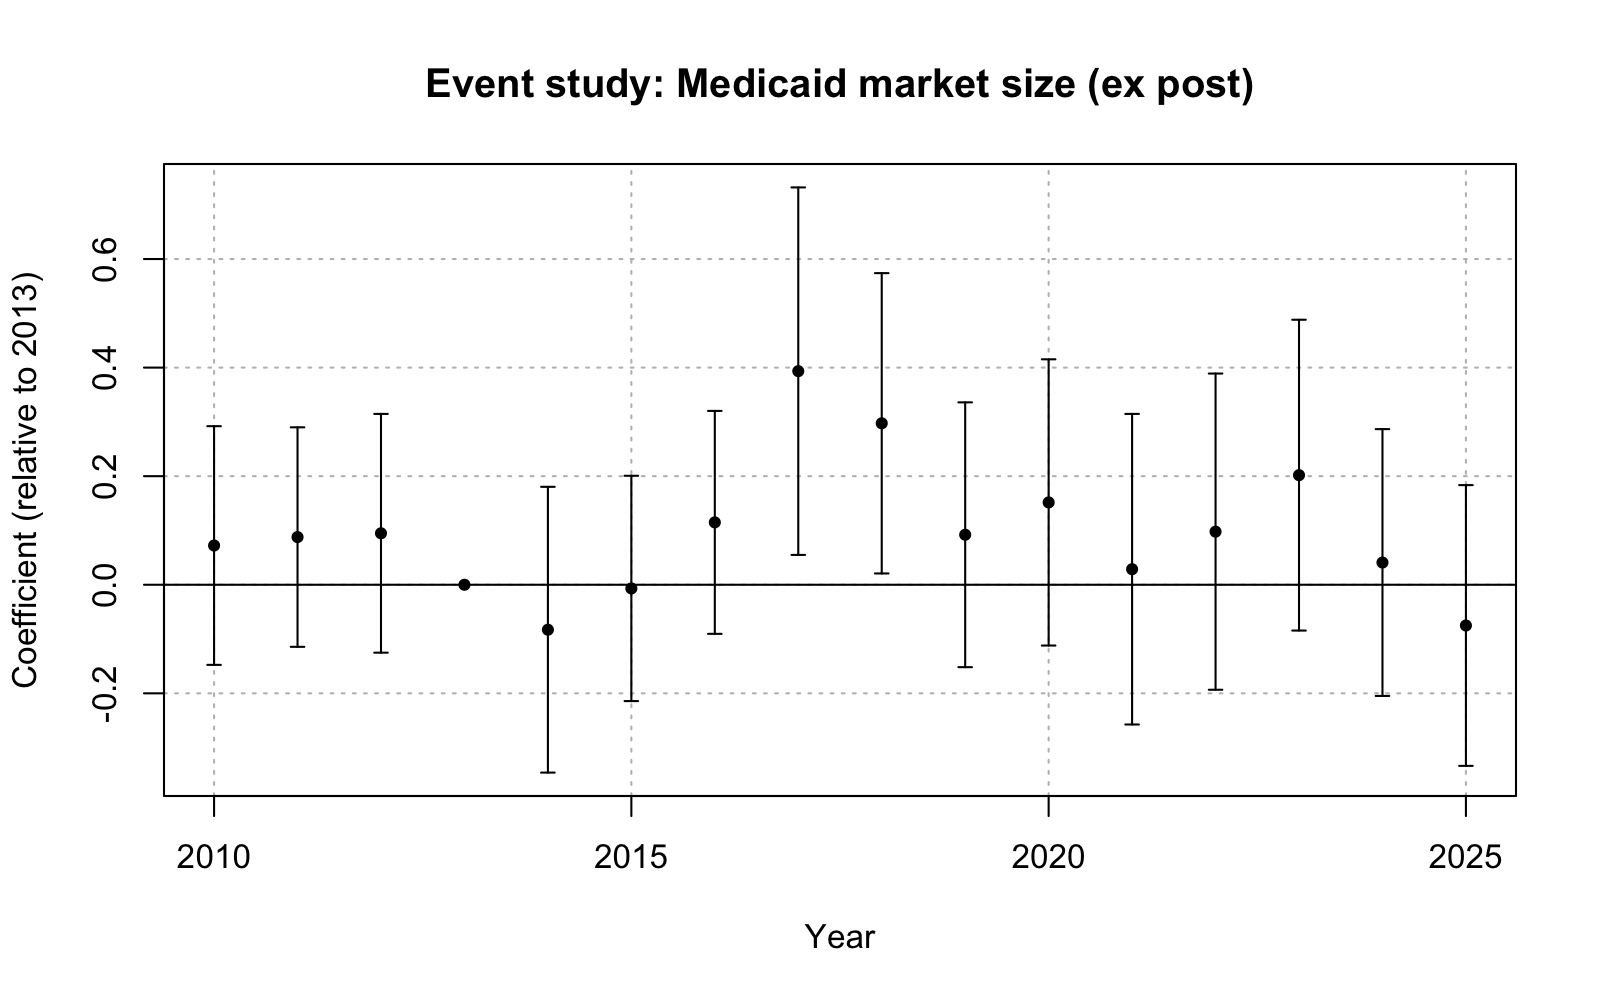
\includegraphics[width=\linewidth]{../output/RQ2/fda_feols_expost_medicaid.png}
  \caption{FEOLS event study: FDA approvals, Medicaid exposure (ex-post)}
  \label{fig:rq2_fda_feols_expost_medicaid}
\end{figure}

\begin{figure}[!h]
  \centering
  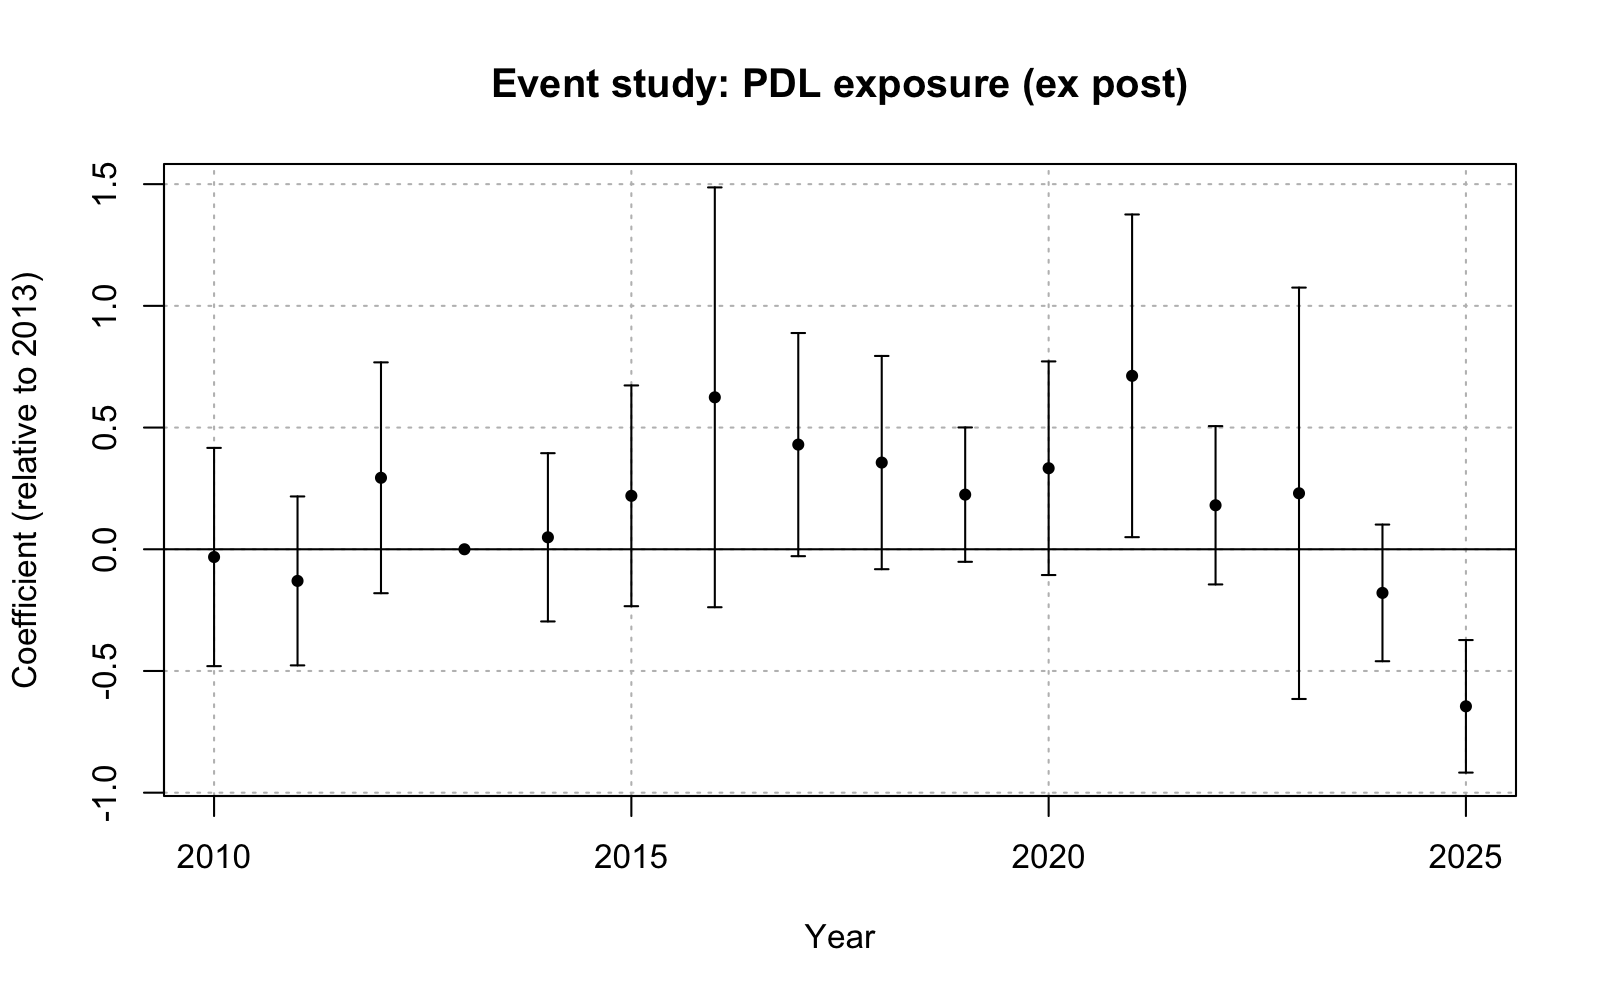
\includegraphics[width=\linewidth]{../output/RQ2/fda_feols_expost_pdl.png}
  \caption{FEOLS event study: FDA approvals, PDL exposure (ex-post)}
  \label{fig:rq2_fda_feols_expost_pdl}
\end{figure}

\clearpage
\begingroup\footnotesize
\begin{table}
\centering
\begin{talltblr}[         %% tabularray outer open
entry=none,label=none,
note{}={* p \num{< 0.05}, ** p \num{< 0.01}, *** p \num{< 0.001}},
]                     %% tabularray outer close
{                     %% tabularray inner open
width=\linewidth,
colspec={Q[]X[]X[]X[]X[]},
column{2,3,4,5}={}{halign=c,},
column{1}={}{halign=l,},
hline{33}={1,2,3,4,5}{solid, black, 0.05em},
}                     %% tabularray inner close
\toprule
& \SetCell[c=2]{c} FEOLS: Ex Ante && \SetCell[c=2]{c} FEOLS: Ex Post & \\
& Medicaid Share & PDL Exposure & Medicaid Share & PDL Exposure \\ \midrule
2010 & \num{0.214}   & \num{0.049}   & \num{0.285}   & \num{0.046}   \\
     & (\num{0.461}) & (\num{0.807}) & (\num{0.448}) & (\num{0.807}) \\
2011 & \num{-0.010}  & \num{-0.243}  & \num{0.344}   & \num{-0.257}  \\
     & (\num{0.382}) & (\num{0.712}) & (\num{0.412}) & (\num{0.711}) \\
2012 & \num{0.171}   & \num{1.402}   & \num{0.371}   & \num{1.395}   \\
     & (\num{0.406}) & (\num{0.911}) & (\num{0.447}) & (\num{0.912}) \\
2014 & \num{-0.333}  & \num{0.403}   & \num{-0.338}  & \num{0.398}   \\
     & (\num{0.465}) & (\num{0.647}) & (\num{0.536}) & (\num{0.647}) \\
2015 & \num{-0.088}  & \num{1.163}   & \num{-0.037}  & \num{1.158}   \\
     & (\num{0.478}) & (\num{0.881}) & (\num{0.422}) & (\num{0.881}) \\
2016 & \num{0.334}   & \num{2.645}   & \num{0.456}   & \num{2.642}   \\
     & (\num{0.426}) & (\num{1.683}) & (\num{0.418}) & (\num{1.682}) \\
2017 & \num{1.364}*  & \num{1.923}   & \num{1.566}*  & \num{1.924}   \\
     & (\num{0.680}) & (\num{0.994}) & (\num{0.690}) & (\num{0.992}) \\
2018 & \num{0.949}   & \num{1.684}   & \num{1.181}*  & \num{1.683}   \\
     & (\num{0.552}) & (\num{1.021}) & (\num{0.563}) & (\num{1.021}) \\
2019 & \num{0.519}   & \num{1.164}*  & \num{0.359}   & \num{1.171}*  \\
     & (\num{0.539}) & (\num{0.592}) & (\num{0.498}) & (\num{0.591}) \\
2020 & \num{0.687}   & \num{1.579}   & \num{0.598}   & \num{1.585}   \\
     & (\num{0.514}) & (\num{0.942}) & (\num{0.537}) & (\num{0.942}) \\
2021 & \num{0.038}   & \num{3.114}*  & \num{0.103}   & \num{3.110}*  \\
     & (\num{0.640}) & (\num{1.394}) & (\num{0.583}) & (\num{1.393}) \\
2022 & \num{0.333}   & \num{0.994}   & \num{0.381}   & \num{0.994}   \\
     & (\num{0.648}) & (\num{0.655}) & (\num{0.593}) & (\num{0.653}) \\
2023 & \num{0.809}   & \num{1.185}   & \num{0.798}   & \num{1.191}   \\
     & (\num{0.649}) & (\num{1.738}) & (\num{0.583}) & (\num{1.737}) \\
2024 & \num{0.272}   & \num{-0.452}  & \num{0.154}   & \num{-0.447}  \\
     & (\num{0.523}) & (\num{0.590}) & (\num{0.501}) & (\num{0.589}) \\
2025 & \num{-0.109}  & \num{-1.118}  & \num{-0.347}  & \num{-1.113}  \\
     & (\num{0.506}) & (\num{0.908}) & (\num{0.525}) & (\num{0.908}) \\
Num. obs. & \num{151200} & & \num{151200} & \\
R2        & \num{0.609}  & & \num{0.609}  & \\
\bottomrule
\end{talltblr}
\end{table}

\endgroup

\clearpage

% -----------------------------------------------------------------------
\section{RQ3: Therapeutic-Class Heterogeneity}
% -----------------------------------------------------------------------

\subsection{Patents}

\begin{center}
\begingroup\footnotesize
\begin{table}
\centering
\begin{talltblr}[         %% tabularray outer open
entry=none,label=none,
note{}={* p \num{< 0.05}, ** p \num{< 0.01}, *** p \num{< 0.001}},
]                     %% tabularray outer close
{                     %% tabularray inner open
colspec={Q[]Q[]Q[]},
column{2,3}={}{halign=c,},
column{1}={}{halign=l,},
hline{26}={1,2,3}{solid, black, 0.05em},
}                     %% tabularray inner close
\toprule
& FEOLS: Ex Ante & FEOLS: Ex Post \\ \midrule
Medicaid Share × ATC = A & \num{-0.165}*** & \num{-0.157}*** \\
& (\num{0.033})   & (\num{0.031})   \\
Medicaid Share × ATC = B & \num{0.134}***  & \num{0.151}***  \\
& (\num{0.024})   & (\num{0.027})   \\
Medicaid Share × ATC = C & \num{-0.123}*** & \num{-0.094}*** \\
& (\num{0.019})   & (\num{0.015})   \\
Medicaid Share × ATC = D & \num{-0.030}    & \num{-0.017}    \\
& (\num{0.108})   & (\num{0.062})   \\
Medicaid Share × ATC = G & \num{0.037}     & \num{0.032}     \\
& (\num{0.056})   & (\num{0.049})   \\
Medicaid Share × ATC = H & \num{0.876}***  & \num{0.619}***  \\
& (\num{0.136})   & (\num{0.096})   \\
Medicaid Share × ATC = J & \num{0.055}     & \num{0.035}     \\
& (\num{0.054})   & (\num{0.034})   \\
Medicaid Share × ATC = L & \num{0.346}     & \num{0.443}     \\
& (\num{0.452})   & (\num{0.578})   \\
Medicaid Share × ATC = M & \num{-0.336}*** & \num{-0.212}*** \\
& (\num{0.076})   & (\num{0.048})   \\
Medicaid Share × ATC = N & \num{-0.125}*** & \num{-0.174}*** \\
& (\num{0.028})   & (\num{0.039})   \\
Medicaid Share × ATC = R & \num{0.005}     & \num{0.005}     \\
& (\num{0.003})   & (\num{0.003})   \\
Medicaid Share × ATC = S & \num{0.093}***  & \num{0.105}***  \\
& (\num{0.017})   & (\num{0.020})   \\
Num. obs.                & \num{19617728}  & \num{19617728}  \\
R2                       & \num{0.247}     & \num{0.247}     \\
\bottomrule
\end{talltblr}
\end{table}

\endgroup
\end{center}

\subsection{FDA Approvals}

\begin{center}
\begingroup\footnotesize
\begin{table}
\centering
\begin{talltblr}[         %% tabularray outer open
entry=none,label=none,
note{}={* p \num{< 0.05}, ** p \num{< 0.01}, *** p \num{< 0.001}},
]                     %% tabularray outer close
{                     %% tabularray inner open
colspec={Q[]Q[]Q[]},
column{2,3}={}{halign=c,},
column{1}={}{halign=l,},
hline{26}={1,2,3}{solid, black, 0.05em},
}                     %% tabularray inner close
\toprule
& FEOLS: Ex Ante & FEOLS: Ex Post \\ \midrule %% TinyTableHeader
Medicaid Share × ATC = A & \num{1.211}** & \num{1.301}** \\
& (\num{0.391}) & (\num{0.420}) \\
Medicaid Share × ATC = B & \num{-0.396}  & \num{-0.121}  \\
& (\num{2.567}) & (\num{0.784}) \\
Medicaid Share × ATC = C & \num{0.229}   & \num{0.373}   \\
& (\num{0.171}) & (\num{0.278}) \\
Medicaid Share × ATC = D & \num{0.707}** & \num{0.881}** \\
& (\num{0.270}) & (\num{0.337}) \\
Medicaid Share × ATC = G & \num{-2.516}  & \num{-1.058}  \\
& (\num{2.666}) & (\num{1.121}) \\
Medicaid Share × ATC = H & \num{1.144}   & \num{0.446}   \\
& (\num{1.358}) & (\num{0.530}) \\
Medicaid Share × ATC = J & \num{-0.145}  & \num{-0.078}  \\
& (\num{0.165}) & (\num{0.089}) \\
Medicaid Share × ATC = L & \num{-0.321}  & \num{-0.244}  \\
& (\num{2.789}) & (\num{2.115}) \\
Medicaid Share × ATC = M & \num{0.022}   & \num{0.017}   \\
& (\num{1.127}) & (\num{0.858}) \\
Medicaid Share × ATC = N & \num{0.034}   & \num{0.047}   \\
& (\num{0.074}) & (\num{0.101}) \\
Medicaid Share × ATC = R & \num{0.298}   & \num{0.178}   \\
& (\num{0.217}) & (\num{0.130}) \\
Medicaid Share × ATC = S & \num{8.052}*  & \num{6.473}*  \\
& (\num{3.737}) & (\num{3.004}) \\
Num. obs.                                           & \num{561600}  & \num{561600}  \\
R2                                                  & \num{0.235}   & \num{0.235}   \\
\bottomrule
\end{talltblr}
\end{table}

\endgroup
\end{center}

\clearpage

% -----------------------------------------------------------------------
\section{PDL Counterfactual Analysis}
% -----------------------------------------------------------------------

\begin{center}
\begingroup\footnotesize
\begin{table}
\centering
\begin{talltblr}[         %% tabularray outer open
entry=none,label=none,
note{}={* p \num{< 0.05}, ** p \num{< 0.01}, *** p \num{< 0.001}},
]                     %% tabularray outer close
{                     %% tabularray inner open
width=\linewidth,
colspec={Q[]X[]X[]},
column{2,3}={}{halign=c,},
column{1}={}{halign=l,},
hline{8}={1,2,3}{solid, black, 0.05em},
}                     %% tabularray inner close
\toprule
& Patents & FDA Approvals \\ \midrule %% TinyTableHeader
Post $\times$ P\&T Pass & \num{-11.399}*  & \num{1.002}   \\
& (\num{4.663})   & (\num{0.633}) \\
Post $\times$ Price Pass & \num{-7.386}*** & \num{0.057}   \\
& (\num{2.173})   & (\num{0.881}) \\
Post $\times$ In PDL & \num{15.549}**  & \num{-0.112}  \\
& (\num{5.215})   & (\num{1.174}) \\
Num. obs.                                 & \num{5281696}   & \num{151200}  \\
R2                                        & \num{0.535}     & \num{0.609}   \\
\bottomrule
\end{talltblr}
\end{table}

\endgroup
\end{center}

\clearpage

\bibliographystyle{apalike}
\bibliography{references}

\end{document}
